\documentclass[a4paper,10pt]{article}

% =========================
%        Packages
% =========================
\usepackage[left=2.5cm, right=2.5cm, top=3cm, bottom=3cm]{geometry}
\usepackage[UTF8]{ctex}
\usepackage{amsmath, amssymb}
\usepackage{booktabs}
\usepackage{array}
\usepackage{graphicx}
\usepackage{float}
\usepackage{hyperref}
\usepackage{xcolor}
\usepackage{listings}
\usepackage{listings}
\usepackage{threeparttable}
\usepackage{multirow} 

% --- code block style ---
\lstset{
    language=Python,
    basicstyle=\ttfamily\footnotesize,
    keywordstyle=\color{blue},
    stringstyle=\color{red},
    commentstyle=\color{green!50!black},
    numbers=left,
    numberstyle=\tiny\color{gray},
    stepnumber=1,
    breaklines=true,
    frame=single,
    backgroundcolor=\color{gray!5},
    showstringspaces=false,
    captionpos=b,
    tabsize=4
}

% =========================
%        Document
% =========================
\begin{document}

% =========================
%        Cover
% =========================
\begin{center}
    \vspace*{1cm}
    {\Huge ZO-1 Capstone 双周报 4}
    
    \vspace{2.2cm}
    {\Large March 29， 2026}
    
    \vspace{1.2cm}
    \renewcommand{\arraystretch}{1.5}
    \begin{tabular}{@{} >{\bfseries}l l @{}}
        \toprule[1.5pt]
        项目企业 & 中欧瑞博 \\
        项目名称 & 股东回报因子探索：考虑净回购的股息率 + 因子 \\
        学生姓名 & 沈可涵 (123090483), 蒋之伟 (123090233), 杨衍韬 (123090731) \\
        报告周期 & 2026 年 3 月 16 日至 2026 年 3 月 29 日 \\
        提交日期 & 2026 年 3 月 29 日 \\
        \bottomrule[1.5pt]
    \end{tabular}
\end{center}

\newpage
\tableofcontents
\newpage

% =========================
%        Main Text
% =========================

\section{大纲与本期更新摘要}



\section{基于国盛证券八分组的港股分类进一步研究——结合财务指标}


在完成前序章节关于企业自由现金流（FCFF）的初步测算以及红利低波基准策略（Benchmark）的构建后，本阶段研究转向深度财务特征分类。我们引入国盛证券的八分组框架，旨在通过内生造血能力与外部融资行为的交叉维度，对港股标的进行精细化刻画。

% ============================================================
\subsection{数据清洗}
% ============================================================

\subsubsection{成交额数据量纲断层}

在对 2010 年至 2025 年全量样本进行回测初步尝试时，我们通过数据诊断表发现，2018 年以前的有效样本量虽然存在，但经过流动性筛选后进入各分组的股票数量极度匮乏。

通过量价交叉验证，即计算理论成交额（收盘价 $\times$ 成交量）与原始名义成交额的比值（Ratio），我们识别出了严重的量纲结构性断层。在 2010 年至 2017 年间，比值中位数高度集中在 1000 附近，说明原始成交额字段以千港元为单位。2018 年为过渡年，千元单位占比降至 61.97\%，而一元单位占比升至 37.22\%。自 2019 年起，一元单位占比稳居 97\% 以上，标志着数据供应商完成了量纲切换。若不进行修复，早期大量蓝筹股会因成交额被低估一千倍而无法通过日均交易量大于一百万港元的门槛，导致回测结果严重失真。

为了防止收盘价上涨拉高估计值，本组摒弃了使用单日的估计交易量与在案数据的比值修正逻辑，而是采用基于自然周的滚动中位数法。该算法通过计算上述比值的周均中位数，有效过滤了单日尾盘异动带来的比值噪音，且能精准定位月中发生的单位切换时点。当周度比值落入 $[900, 1100]$ 区间时，系统自动对该周 \texttt{amount} 字段乘以 1000 进行大致还原，以防止误过滤。

\subsubsection{利润表计价货币单位问题}

在计算盈利收益率（EP）与资本回报率（ROIC）等跨表财务因子时，由于港股市场的国际化特征，上市公司的底层财务报表存在多种计价货币（如港币 HKD、人民币 CNY、美元 USD 等）。特别是在计算 EP（$EP = \text{净利润} / \text{总市值}$）时，由于底层行情表提供的总市值统一以港币计价，若直接使用原始利润表中的归母净利润字段（\texttt{NP\_BELONGTO\_COMMONSH}）相除，会导致极其严重的量纲与币种错配。例如，大量以内地业务为主的红筹股与 H 股以人民币（CNY）披露财报，若不进行汇率换算，其 EP 因子值将被系统性低估，进而导致在后续 EP-ROIC 横截面排序中产生严重偏差。

为解决这一跨表量纲错配问题，本研究在财务数据清洗阶段引入了常数汇率转换矩阵（FX Mapping）。算法通过提取利润表中的货币代码字段（\texttt{CRNCY\_CODE}），将所有非港币计价的净利润严格映射并折算为统一的港币口径。本研究共覆盖 17 种货币，主要映射关系如表~\ref{tab:fx_mapping} 所示。所有财务绝对值指标在完成统一折算后，再与市值数据进行对齐与除法运算，排除了货币种类不匹配导致的影响。

\begin{table}[H]
\centering
\caption{主要货币兑港币汇率映射（常数近似）}
\label{tab:fx_mapping}
\small
\begin{tabular}{llllll}
\toprule
货币 & 兑HKD & 货币 & 兑HKD & 货币 & 兑HKD \\
\midrule
HKD & 1.000 & SGD & 5.800 & JPY & 0.052 \\
CNY & 1.080 & MYR & 1.750 & AUD & 5.000 \\
USD & 7.800 & EUR & 8.500 & CAD & 5.700 \\
MOP & 0.970 & GBP & 9.900 & TWD & 0.240 \\
KRW & 0.0057 & THB & 0.220 & IDR & 0.00049 \\
ZAR & 0.420 & RUB & 0.086 & — & — \\
\bottomrule
\end{tabular}
\end{table}

% ============================================================
\subsection{八分组逻辑定义与特征画像}
% ============================================================

基于修复后的清洁数据，我们利用 FCFF 覆盖度、股权融资及债权融资三个维度构建八分组模型。分类依据如下表所示：

\begin{table}[H]
\centering
\caption{股东回报八分组分类依据及财务特征}
\label{tab:eight_groups}
\small
\begin{tabular}{lp{1.8cm}p{1.8cm}p{1.8cm}p{4.5cm}}
\toprule
组别 & FCFF覆盖度 & 股权融资 & 债权融资 & 直觉财务画像 \\
\midrule
Group 1 & True  & False & False & 内生造血极强，无外部依赖 \\
Group 2 & True  & False & True  & 现金流充裕，通过债务扩张 \\
Group 3 & True  & True  & False & 现金流健康，伴随股权扩张 \\
Group 4 & True  & True  & True  & 内生外行双轮驱动 \\
Group 5 & False & False & False & 现金流不足，消耗存量储备 \\
Group 6 & False & False & True  & 借债维持回报或运营 \\
Group 7 & False & True  & False & 股权稀释型分红/运营 \\
Group 8 & False & True  & True  & 极度依赖外部输血 \\
\bottomrule
\end{tabular}
\end{table}

\subsubsection{八分组核心指标的计算逻辑}

为了确保全市场数据的可比性，本研究中八分组模型的所有底层指标均通过现金流量表（Cash Flow Statement）推导得出。具体计算公式与科目对应如下：

\paragraph{自由现金流（FCFF）}
根据流量法视角的重构，企业自由现金流（FCFF）可通过以下公式计算：
\begin{equation}
FCFF = \text{经营活动现金流净额} + \text{利息支出} - \text{资本性支出}
\end{equation}
其中，各变量对应中国会计准则或国际财务报告准则（IFRS）现金流量表中的具体科目：
\begin{itemize}
    \item \textbf{经营活动现金流净额}：直接取自"经营活动产生的现金流量净额"。
    \item \textbf{资本性支出 (CapEx)}：取"购建固定资产、无形资产和其他长期资产支付的现金"减去"处置固定资产、无形资产和其他长期资产收回的现金净额"。
    \item \textbf{利息支出}：由于 A 股/港股财报常将其与分红合并，此处通过"分配股利、利润或偿付利息支付的现金"减去"当年实际分红金额"间接倒算得出。
\end{itemize}

\paragraph{FCFF 覆盖度}
股东回报的总体规模由"分红 + 回购"构成。FCFF 覆盖度即判定公司当年的内生自由现金流是否足以支撑其对股东的实际分配：
\begin{equation}
\text{FCFF 覆盖度} =
\begin{cases}
\text{True},  & \text{若 } FCFF > (\text{实际分红金额} + \text{实际回购金额}) \\
\text{False}, & \text{若 } FCFF \le (\text{实际分红金额} + \text{实际回购金额})
\end{cases}
\end{equation}

\paragraph{外源融资行为}
管理层的资本配置动机通过是否有新增的股权或债权融资来刻画：
\begin{itemize}
    \item \textbf{股权融资}：对应现金流量表中的"吸收投资所得现金"。若该科目金额大于零，则视为存在新增股权融资，标记为 True。
    \item \textbf{债权融资}：取"取得借款所得现金"加"发行债券所得现金"。若当年存在通过举债获取现金的行为，则表明公司可能在利用财务杠杆，标记为 True。
\end{itemize}

综上，上述三个维度（FCFF 是否覆盖、是否有股权融资、是否有债权融资）通过布尔值的排列组合，正交地将实施了股东回报的企业划分为 8 种不同的资本配置模式。

% ============================================================
\subsection{回测绩效与 IC 检验}
% ============================================================

\subsubsection{核心数据基准}

本研究构建了两套平行的信号对齐机制：

\begin{itemize}
    \item \textbf{动态调仓}：在每个月末，基于该时刻市场上已绝对公开披露的最新财报数据滚动换仓，实现对财报发布节奏的最大化利用。
    \item \textbf{静态调仓}：基于法定披露限期（港股财年结束后四个月，即来年四月三十日）进行年度定期对齐，彻底屏蔽因财报延期带来的前视偏差。
\end{itemize}

收益率计算统一使用复权收盘价（AdjClose）的对数收益率，确保分红与拆股事件对回报的影响得到完整反映。月度换仓采用月末最后一个交易日持仓截面，下月收益为下一月末的月度价格变化。

\subsubsection{动态调仓各分组 CAGR 表现}

\begin{table}[H]
\centering
\caption{动态对齐各分组复合年化收益率对比表（2011--2025）}
\label{tab:dynamic_full}
\begin{tabular}{lrr}
\toprule
组别 (Group) & 等权 CAGR & 市值加权 CAGR \\
\midrule
Group 1 &  3.25\% &  6.21\% \\
Group 2 &  5.72\% &  6.34\% \\
Group 3 & -2.15\% &  0.05\% \\
Group 4 &  0.83\% &  6.41\% \\
Group 5 & -0.10\% &  0.21\% \\
Group 6 &  2.24\% &  4.36\% \\
Group 7 &  0.10\% & -5.68\% \\
Group 8 &  0.04\% &  2.96\% \\
\bottomrule
\end{tabular}
\end{table}

% 注释：此处插入动态回测各分组累计净值与回撤走势图，文件名建议 output2.png
\begin{figure}[H]
    \centering
    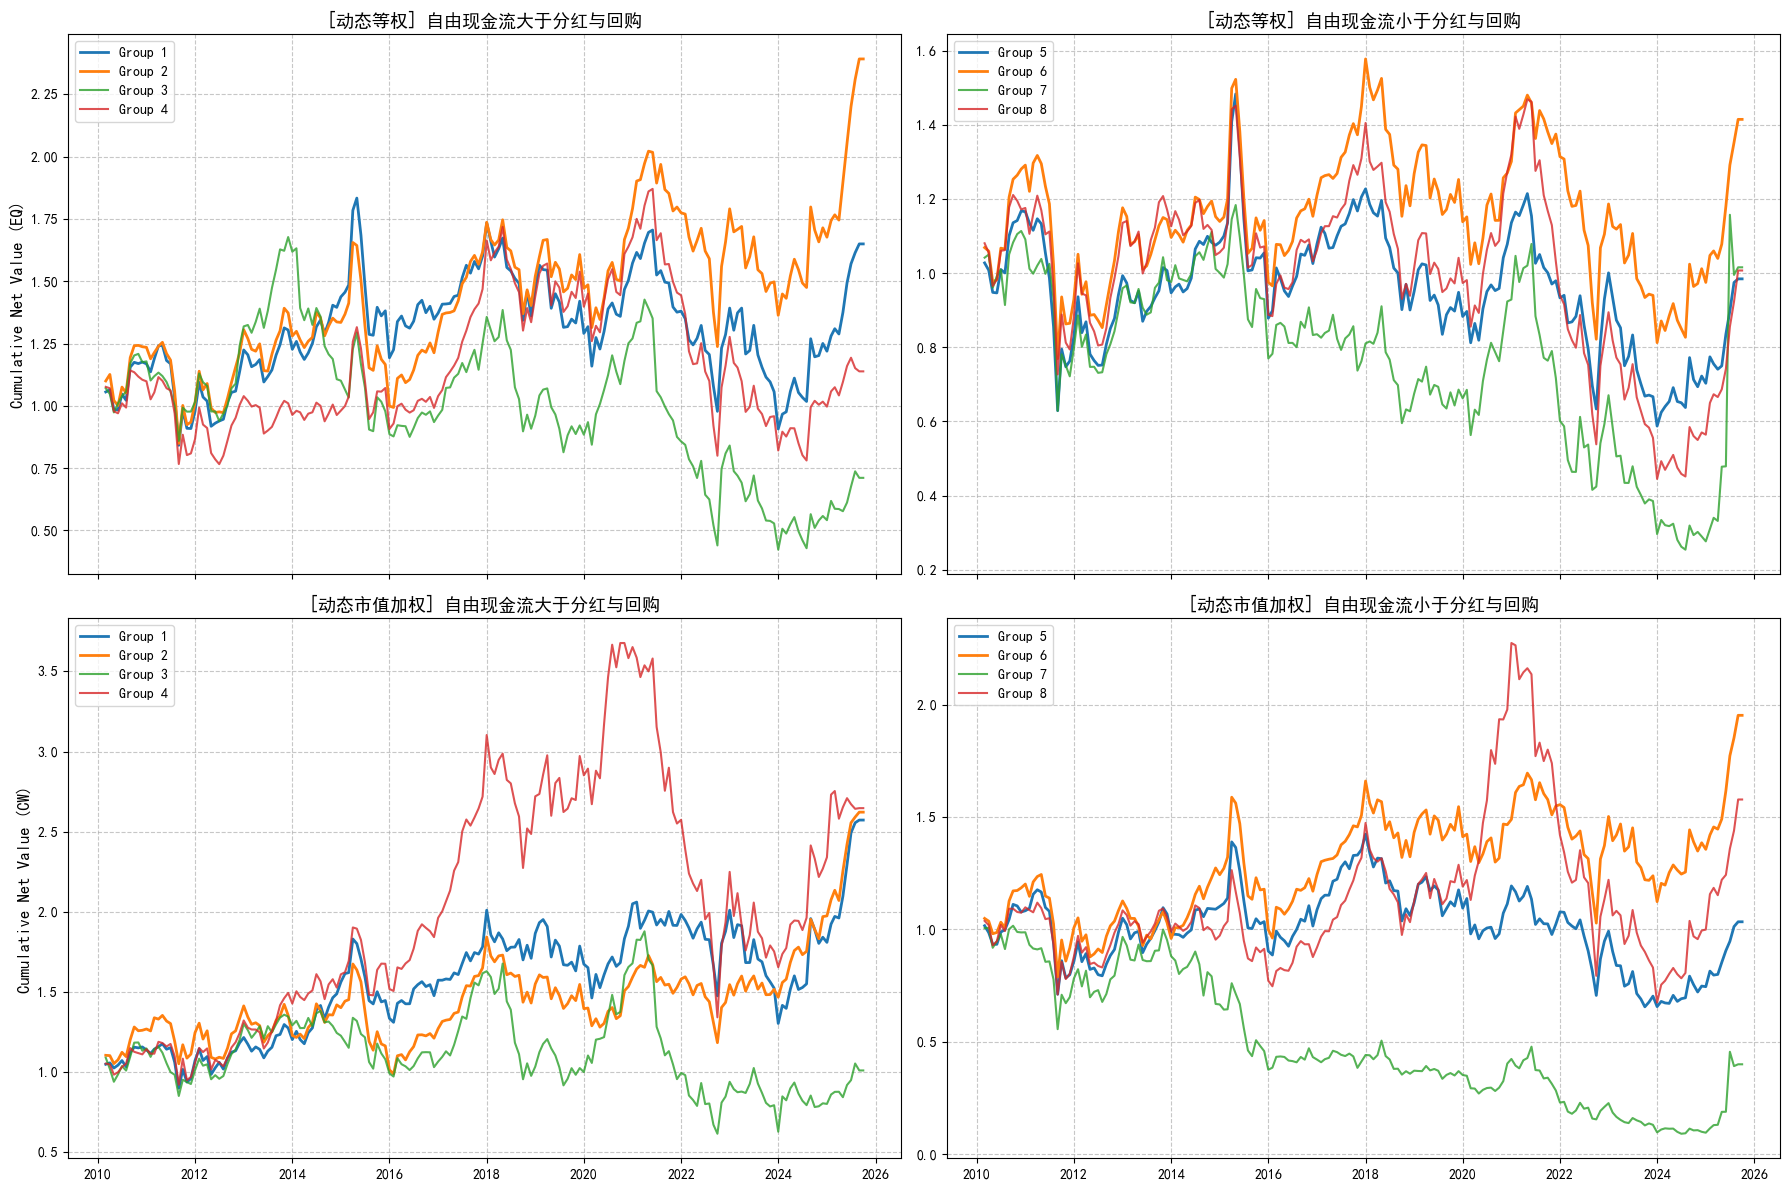
\includegraphics[width=0.95\textwidth]{动态等权.png}
    \caption{动态调仓模式下各分组累计净值与回撤走势图}
    \label{fig:dynamic_plot}
\end{figure}

\subsubsection{静态调仓各分组 CAGR 表现}

\begin{table}[H]
\centering
\caption{静态对齐各分组复合年化收益率对比表（2011--2025）}
\label{tab:static_full}
\begin{tabular}{lrr}
\toprule
组别 (Group) & 等权 CAGR & 市值加权 CAGR \\
\midrule
Group 1 & -0.64\% &  3.64\% \\
Group 2 &  4.16\% &  5.57\% \\
Group 3 & -3.12\% &  0.99\% \\
Group 4 &  0.52\% &  5.92\% \\
Group 5 & -0.21\% &  0.09\% \\
Group 6 &  0.11\% &  2.40\% \\
Group 7 & -8.04\% & -13.76\% \\
Group 8 & -2.35\% &  0.76\% \\
\bottomrule
\end{tabular}
\end{table}

% 注释：此处插入静态回测各分组累计净值与回撤走势图，文件名建议 output1.png
\begin{figure}[H]
    \centering
    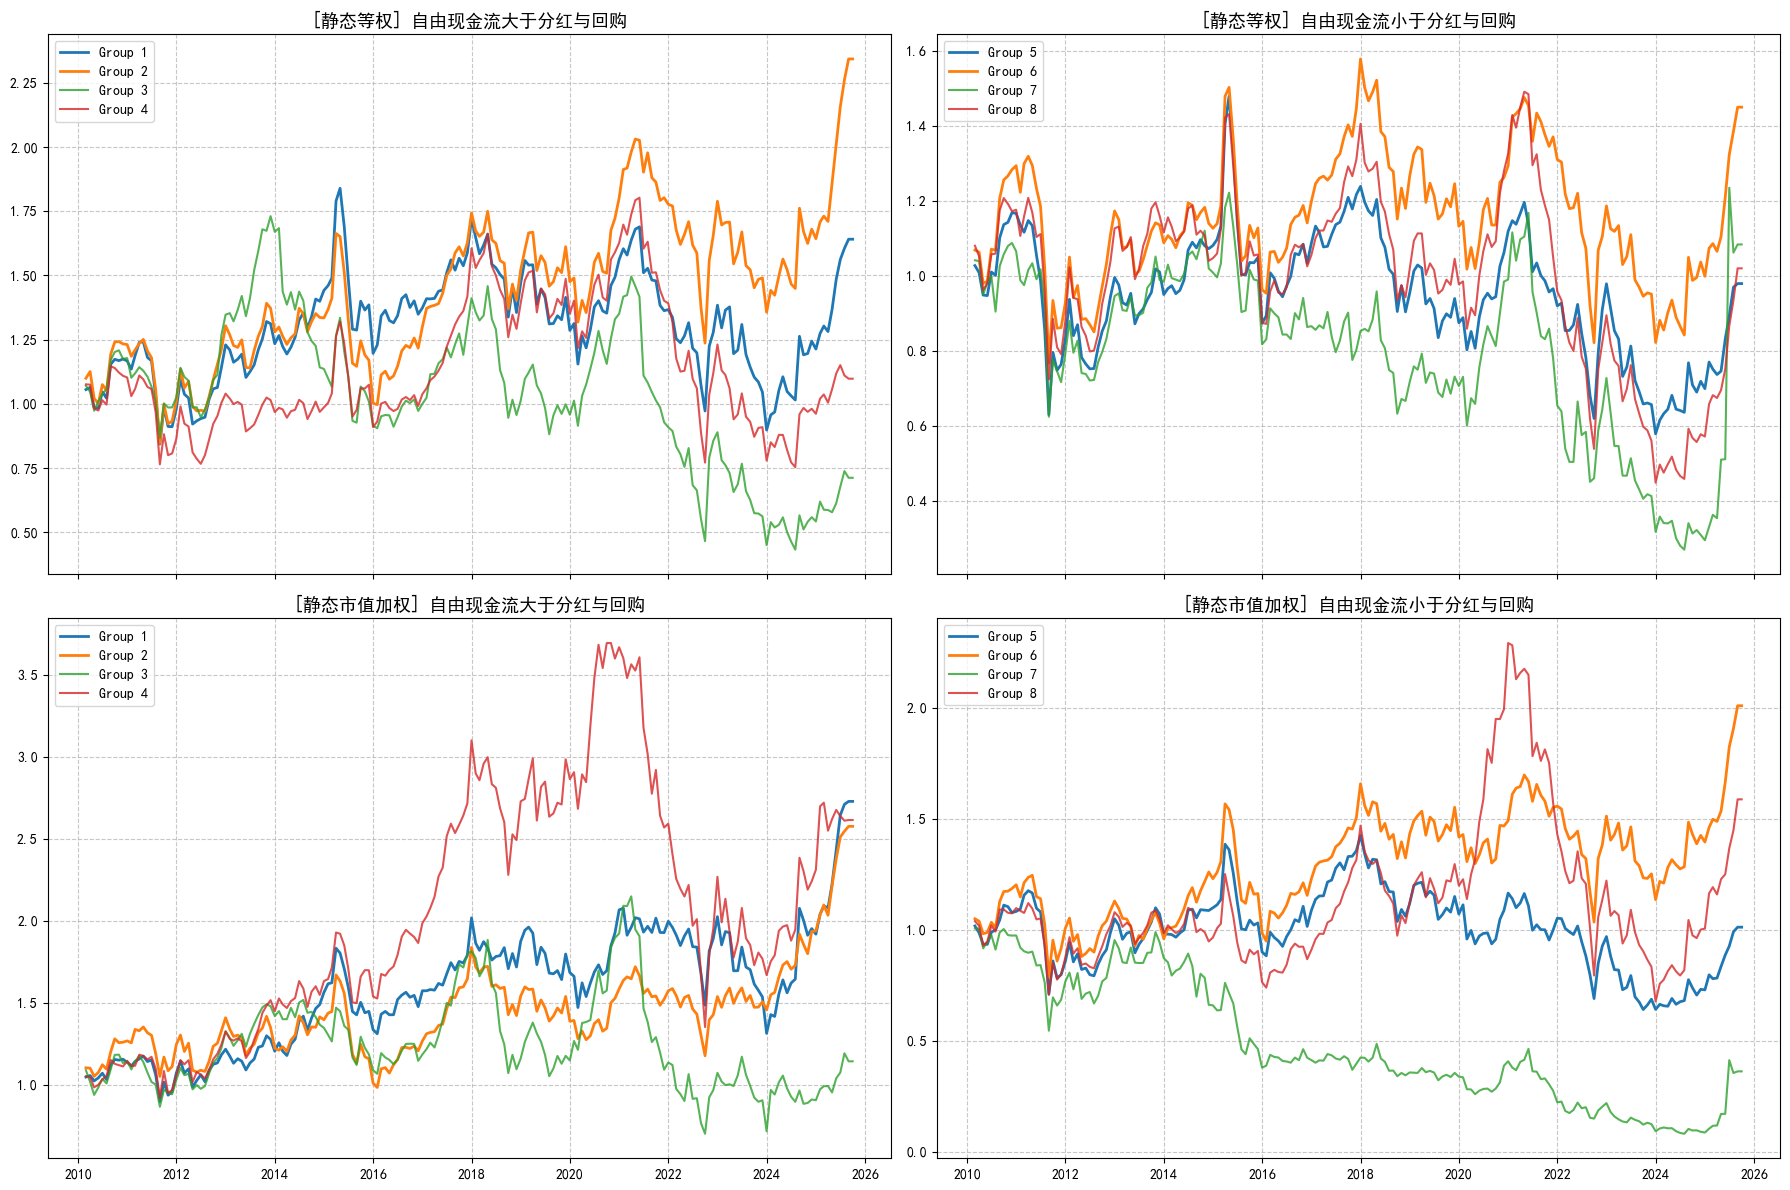
\includegraphics[width=0.95\textwidth]{静态等权.png}
    \caption{静态调仓模式下各分组累计净值与回撤走势图}
    \label{fig:static_plot}
\end{figure}

\subsubsection{IC 检验}

\subsubsubsection{动态回测 IC}

为进一步严谨论证上述收益分化的稳健性，本研究引入了信息系数检验（IC，Spearman 秩相关）。整体截面 IC 以分组编号（1--8）作为序数因子，与次月截面收益率进行 Spearman 相关，并通过 Newey-West HAC 方法修正自相关偏误。

测算表明，整体截面 IC 均值为 $-0.0245$（NW $t$-stat 为 $-4.4382$，高度显著）。因组别编号越小代表基本面越健康，极显著的负值完美印证了"分组编号越小，下月收益越高"的底层逻辑。

\begin{table}[H]
    \centering
    \caption{动态回测各分组条件 IC 检验统计量（全部八组）}
    \label{tab:ic_stats_dyn}
    \begin{tabular}{lrrrr}
        \toprule
        \textbf{组别} & \textbf{IC Mean} & \textbf{IC IR} & \textbf{NW $t$-stat} & \textbf{$p$-value} \\
        \midrule
        Group 1 &  0.0081 &  0.1434 &  2.2353 & 0.0254 \\
        Group 2 &  0.0197 &  0.2886 &  3.9863 & 0.0001 \\
        Group 3 & -0.0066 & -0.1001 & -1.3800 & 0.1676 \\
        Group 4 & -0.0008 & -0.0133 & -0.1407 & 0.8881 \\
        Group 5 & -0.0051 & -0.1019 & -1.4981 & 0.1341 \\
        Group 6 &  0.0000 &  0.0007 &  0.0096 & 0.9923 \\
        Group 7 & -0.0163 & -0.2599 & -3.5421 & 0.0004 \\
        Group 8 & -0.0164 & -0.2328 & -2.9204 & 0.0035 \\
        \bottomrule
    \end{tabular}
\end{table}

Group 2（内生造血+适度举债）展现了全场最强的预测能力（$t$-stat $= 3.99$），Group 1 紧随其后。Group 3--6 的条件 IC 均不显著（$|t| < 1.5$，$p > 0.13$），说明这四组的归属对截面收益的增量预测力接近于零。Group 7 与 Group 8 的条件 IC 均为极显著负值，统计上证实了"股权稀释 + FCFF 不足"是港股长期跑输的核心特征。

表~\ref{tab:ic_corr_dyn} 展示了各分组条件 IC 时间序列之间的 Pearson 相关系数，揭示了分组信号的正交性结构。

\begin{table}[H]
    \centering
    \caption{动态回测各分组条件 IC 时间序列相关矩阵}
    \label{tab:ic_corr_dyn}
    \scriptsize
    \begin{tabular}{lrrrrrrrr}
        \toprule
        & G1 & G2 & G3 & G4 & G5 & G6 & G7 & G8 \\
        \midrule
        G1 &  1.00 &  0.06 & -0.03 & -0.02 & -0.05 & -0.24 & -0.08 & -0.42 \\
        G2 &  0.06 &  1.00 & -0.40 & -0.22 & -0.12 &  0.11 & -0.40 & -0.59 \\
        G3 & -0.03 & -0.40 &  1.00 &  0.12 & -0.04 & -0.38 &  0.26 &  0.17 \\
        G4 & -0.02 & -0.22 &  0.12 &  1.00 & -0.28 & -0.53 &  0.09 & -0.03 \\
        G5 & -0.05 & -0.12 & -0.04 & -0.28 &  1.00 &  0.09 &  0.07 & -0.15 \\
        G6 & -0.24 &  0.11 & -0.38 & -0.53 &  0.09 &  1.00 & -0.38 & -0.18 \\
        G7 & -0.08 & -0.40 &  0.26 &  0.09 &  0.07 & -0.38 &  1.00 &  0.20 \\
        G8 & -0.42 & -0.59 &  0.17 & -0.03 & -0.15 & -0.18 &  0.20 &  1.00 \\
        \bottomrule
    \end{tabular}
\end{table}

G1 与 G8 的 IC 相关系数为 $-0.42$，G2 与 G8 为 $-0.59$，体现了两端分组信号的天然对冲关系——同一时期 G1/G2 表现好时，G8 往往表现差，因子的"多空结构"具有统计支撑。

% 注释：此处插入动态回测月度截面IC柱状图与各分组累计条件IC走势图，文件名建议 pic1.png
\begin{figure}[H]
    \centering
    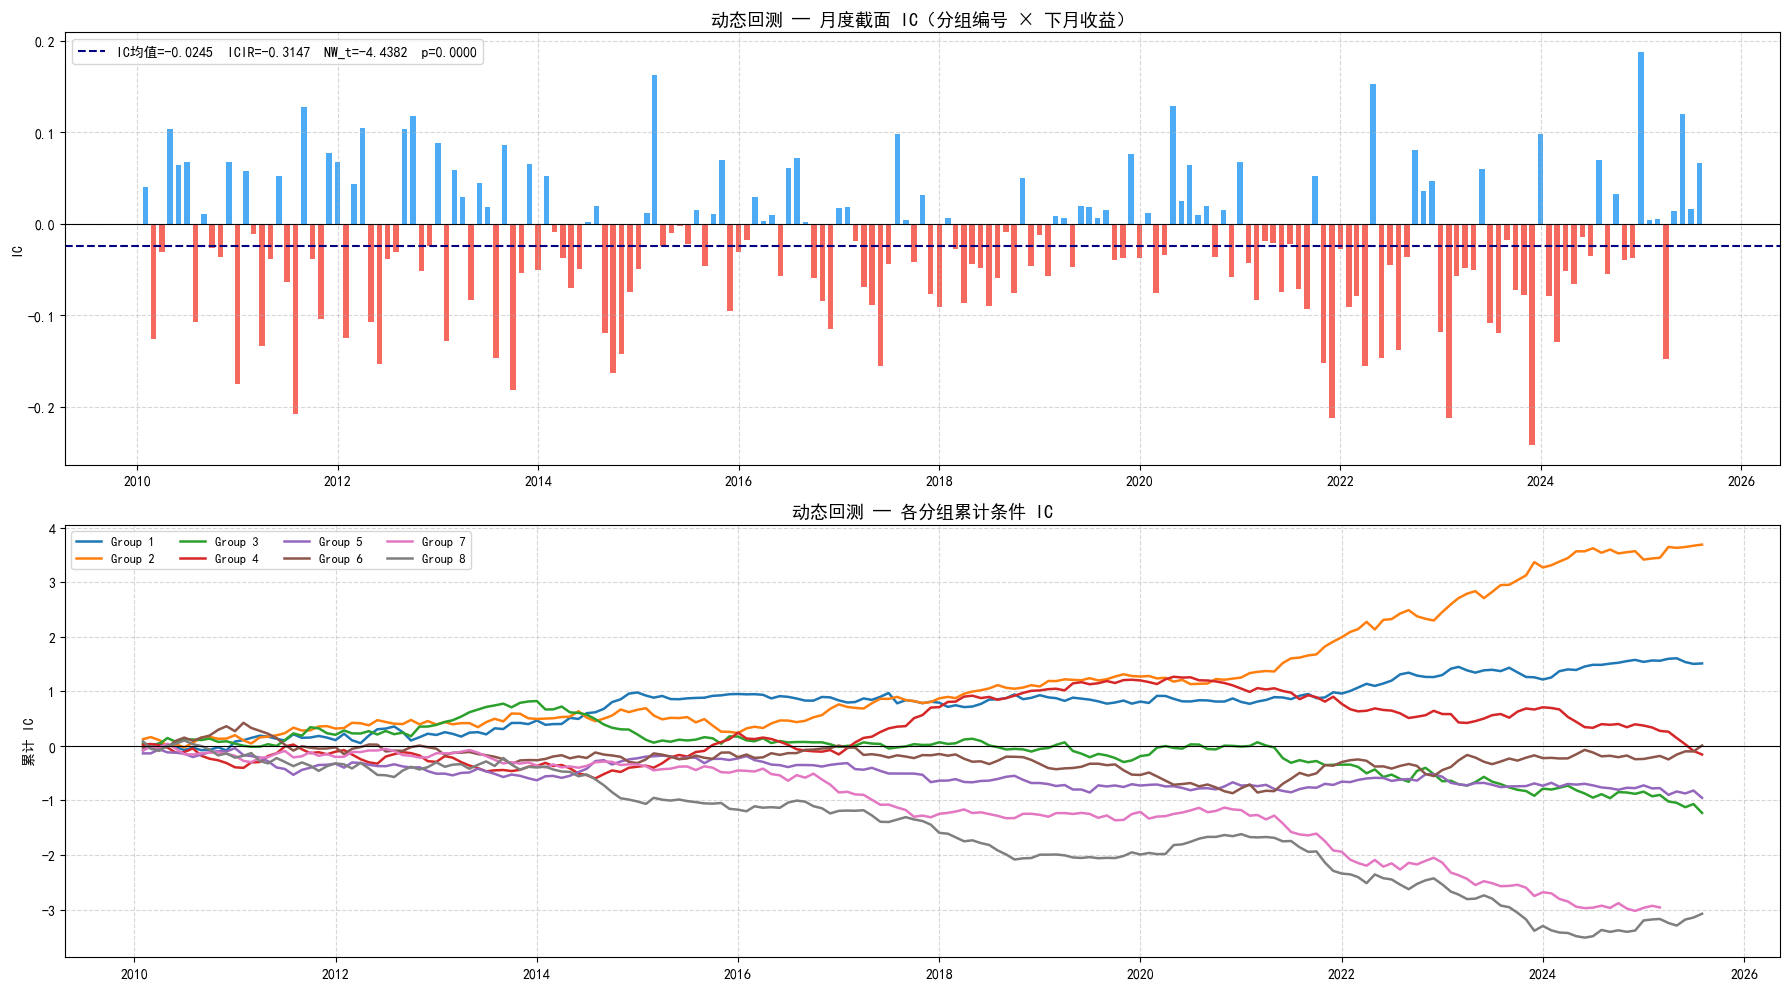
\includegraphics[width=0.90\textwidth]{动态回测.png}
    \caption{动态回测：月度截面 IC（上）与各分组累计条件 IC 走势（下）}
    \label{fig:ic_trend_dyn}
\end{figure}

\subsubsubsection{静态回测 IC}

静态调仓模式下，整体截面 IC 均值为 $-0.0241$（ICIR $= -0.3000$，NW $t$-stat $= -4.3306$，$p = 0.0000$），与动态模式高度一致，表明分组信号的预测效力不依赖于财报对齐方式。

\begin{table}[H]
    \centering
    \caption{静态回测各分组条件 IC 检验统计量（全部八组）}
    \label{tab:ic_stats_stat}
    \begin{tabular}{lrrrr}
        \toprule
        \textbf{组别} & \textbf{IC Mean} & \textbf{IC IR} & \textbf{NW $t$-stat} & \textbf{$p$-value} \\
        \midrule
        Group 1 &  0.0044 &  0.0708 &  0.9866 & 0.3238 \\
        Group 2 &  0.0193 &  0.2818 &  3.9171 & 0.0001 \\
        Group 3 & -0.0048 & -0.0705 & -0.9468 & 0.3438 \\
        Group 4 &  0.0035 &  0.0535 &  0.5728 & 0.5668 \\
        Group 5 & -0.0018 & -0.0343 & -0.5111 & 0.6093 \\
        Group 6 & -0.0024 & -0.0342 & -0.4401 & 0.6598 \\
        Group 7 & -0.0171 & -0.2598 & -3.4739 & 0.0005 \\
        Group 8 & -0.0170 & -0.2373 & -3.0262 & 0.0025 \\
        \bottomrule
    \end{tabular}
\end{table}

静态模式下 Group 1 的条件 IC（$t = 0.99$，$p = 0.32$）统计上不显著，与动态模式（$t = 2.24$，$p = 0.025$）形成对比。这说明 Group 1 的超额收益具有时效性——当财报信号距离持仓时点较远（年度硬截止对齐）时，Group 1 的预测效力有所衰减；Group 2 则在两种模式下均保持高度显著（静态 $t = 3.92$），信号稳健性更强。

\begin{table}[H]
    \centering
    \caption{静态回测各分组条件 IC 时间序列相关矩阵}
    \label{tab:ic_corr_stat}
    \scriptsize
    \begin{tabular}{lrrrrrrrr}
        \toprule
        & G1 & G2 & G3 & G4 & G5 & G6 & G7 & G8 \\
        \midrule
        G1 &  1.00 &  0.05 & -0.03 &  0.02 &  0.06 & -0.27 & -0.11 & -0.36 \\
        G2 &  0.05 &  1.00 & -0.32 & -0.23 & -0.02 &  0.09 & -0.39 & -0.60 \\
        G3 & -0.03 & -0.32 &  1.00 &  0.06 & -0.24 & -0.34 &  0.27 &  0.15 \\
        G4 &  0.02 & -0.23 &  0.06 &  1.00 & -0.24 & -0.52 &  0.09 & -0.05 \\
        G5 &  0.06 & -0.02 & -0.24 & -0.24 &  1.00 & -0.01 &  0.04 & -0.11 \\
        G6 & -0.27 &  0.09 & -0.34 & -0.52 & -0.01 &  1.00 & -0.32 & -0.20 \\
        G7 & -0.11 & -0.39 &  0.27 &  0.09 &  0.04 & -0.32 &  1.00 &  0.17 \\
        G8 & -0.36 & -0.60 &  0.15 & -0.05 & -0.11 & -0.20 &  0.17 &  1.00 \\
        \bottomrule
    \end{tabular}
\end{table}

静态与动态的相关矩阵结构高度相似，G2 与 G8 之间的强负相关（静态 $-0.60$，动态 $-0.59$）在两种模式下均稳定存在，进一步确认了八分组信号的多空结构不依赖于财报对齐方式。

% 注释：此处插入静态回测月度截面IC柱状图与各分组累计条件IC走势图，文件名建议 pic3.png
\begin{figure}[H]
    \centering
    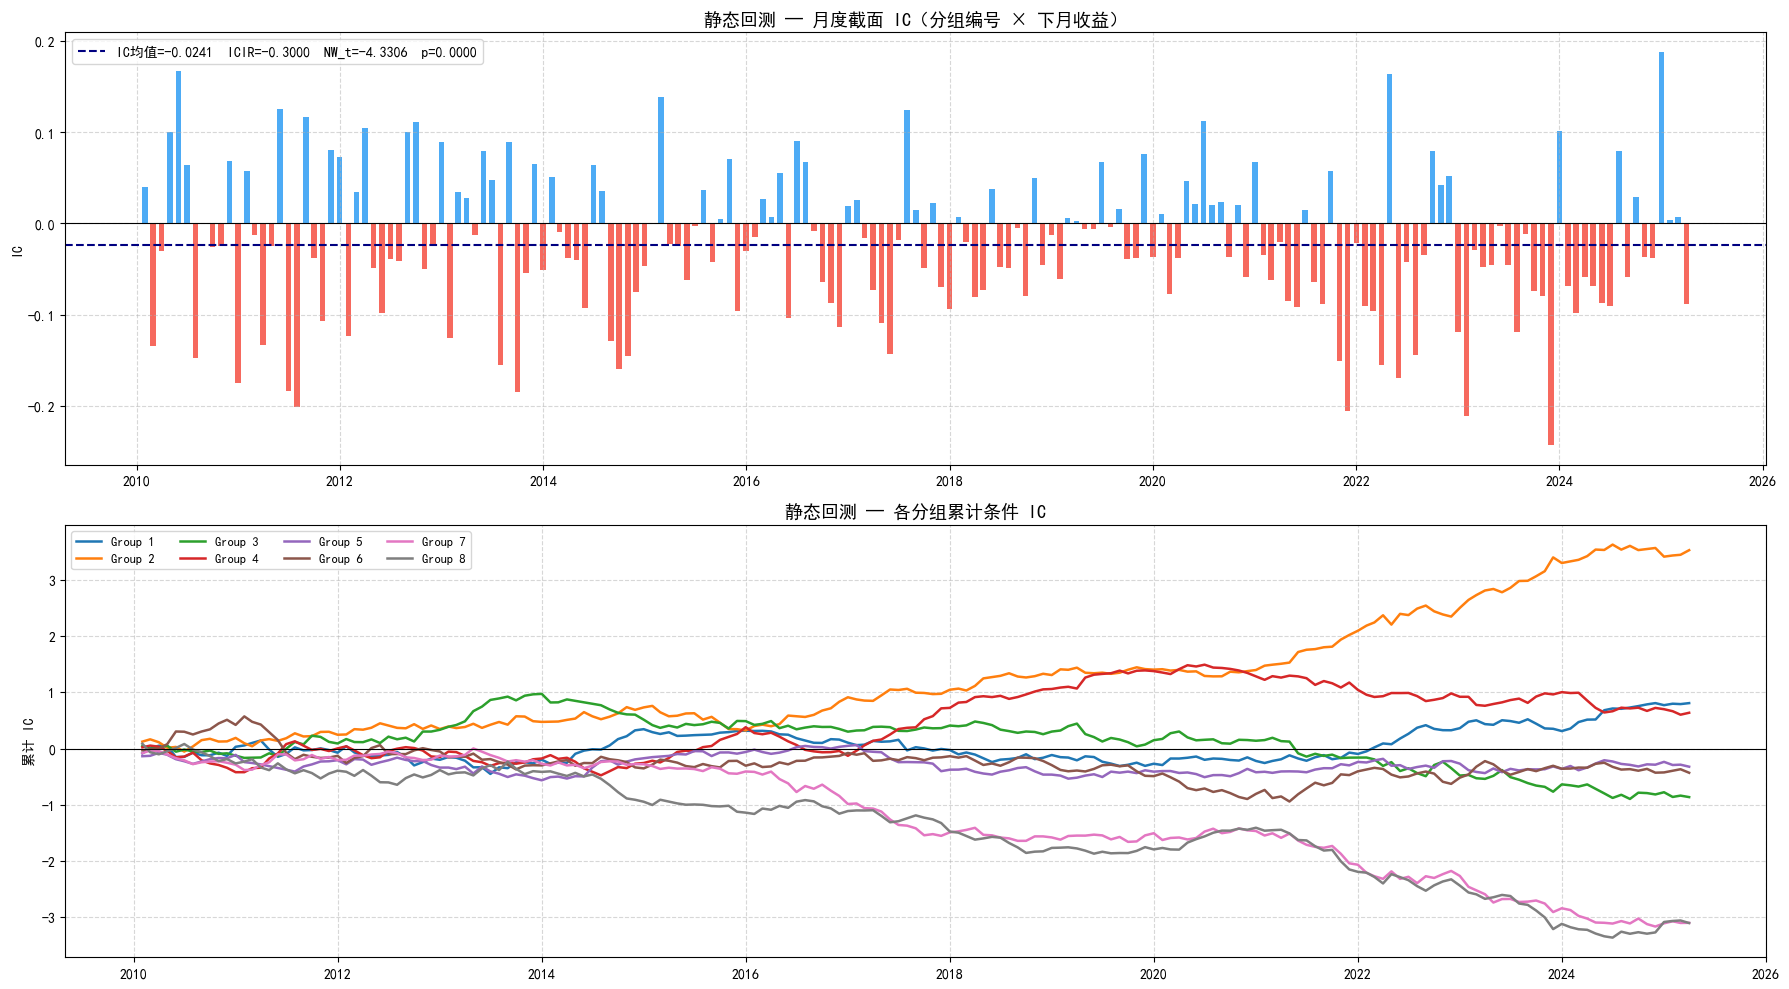
\includegraphics[width=0.90\textwidth]{静态回测.png}
    \caption{静态回测：月度截面 IC（上）与各分组累计条件 IC 走势（下）}
    \label{fig:ic_trend_stat}
\end{figure}

% ============================================================
\subsection{二次特征筛选：波动率与 EP-ROIC 利差的增量贡献}
% ============================================================

基于 Group 1 与 Group 2 的高胜率，本研究进一步检验：在此优质底池中叠加低波动率（防守特征）与高 EP-ROIC 利差（深度价值特征），能否筛选出表现更优的子组合。

具体实现上，以动态回测中 Group 1 与 Group 2 的月度截面成份股为母池（月均约 140 只），分别构建两个二级筛选板块：

\begin{itemize}
    \item \textbf{板块 A（低波动率）}：计算母池内各股 252 日年化波动率（采用复权收盘价 AdjClose 的对数收益率，与回测收益率口径保持一致），取截面分位数后 50\% 的低波动股票。月均持仓约 70 只。
    \item \textbf{板块 B（EP-ROIC 利差）}：对母池内各股的截面 EP 与 ROIC 分别进行双端 1\% Winsorize 处理后，计算差值 $\text{spread} = EP_w - ROIC_w$，取截面差值分位数前 50\% 的股票（纯排名，不加正值门槛，遵循国盛原始框架的连续排序逻辑）。月均持仓约 67 只。
\end{itemize}

值得注意的是，上述两项指标的口径一致性是结果可信的关键前提：波动率使用复权价格以消除除息日跳空噪音；财务数据有效期设定为 550 天上限，以覆盖港股年报最晚次年四月三十日的法定披露期限。

\begin{table}[H]
\centering
\caption{Group 1/2 母池及二次筛选板块 CAGR 对比（2011--2025）}
\label{tab:panel_cagr}
\begin{tabular}{lrr}
\toprule
策略 & 等权 CAGR & 市值加权 CAGR \\
\midrule
\multicolumn{3}{l}{\textit{母池参考基准}} \\
\quad Group 1（动态） &  3.25\% &  6.21\% \\
\quad Group 2（动态） &  5.72\% &  6.34\% \\
\midrule
\multicolumn{3}{l}{\textit{二次筛选板块}} \\
\quad 板块 A（低波动率，截面后 50\%）    & 5.41\% & 6.30\% \\
\quad 板块 B（EP-ROIC 高差值，截面前 50\%）& 5.81\% & \textbf{7.46\%} \\
\bottomrule
\end{tabular}
\end{table}

% 注释：此处插入 Group 1/2 板块A与板块B四轨（等权/市值加权×板块A/B）NAV对比图（2×2子图），
%       文件名建议 pic2.png，由 Cell 6 第 J 段代码生成
\begin{figure}[H]
    \centering
    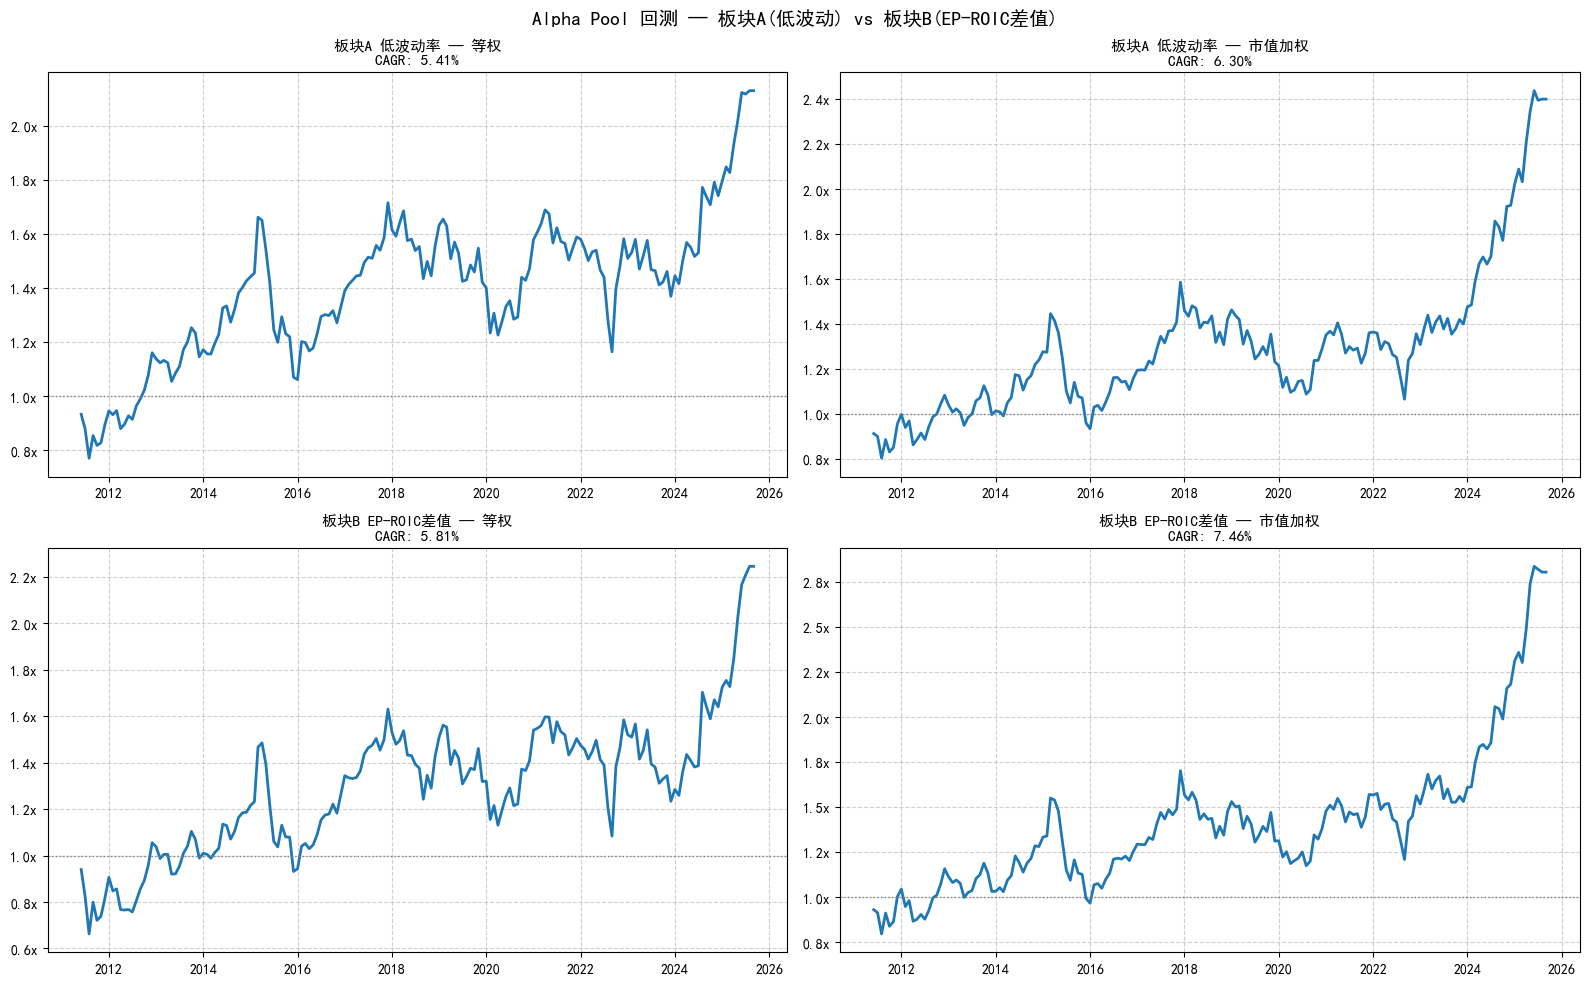
\includegraphics[width=\textwidth]{板块AB.png}
    \caption{Group 1/2 内部二次特征筛选：板块A（低波动率）与板块B（EP-ROIC利差），各含等权与市值加权两轨}
    \label{fig:panel_nav}
\end{figure}

\subsubsection{低波动筛选：降噪有余，增收有限}

板块 A 等权 CAGR 为 5.41\%，显著高于 Group 1 等权（3.25\%），但与 Group 2 等权（5.72\%）接近；市值加权 CAGR 为 6.30\%，与 Group 1/2 各自的市值加权水平（6.21\%/6.34\%）基本持平。

低波动筛选的主要贡献体现在\textbf{等权口径下的组合提升}：母池中 Group 1 的低 CAGR（3.25\% EW）在很大程度上来源于若干高波动小市值股票的拖累，低波动筛选有效屏蔽了这类"波动率贡献大、超额贡献小"的标的，使等权组合向 Group 2 的质量水平看齐。然而在市值加权口径下，大市值蓝筹股天然具有较低波动率，因此低波动筛选对市值加权结果的边际改善接近于零。

\subsubsection{EP-ROIC 利差筛选：价值-质量利差的有效信号}

板块 B 的结果更为突出：等权 CAGR 5.81\% 接近 Group 2 水平（5.72\%），而\textbf{市值加权 CAGR 高达 7.46\%，超越 Group 1（6.21\%）与 Group 2（6.34\%）各自的市值加权表现约 1.1--1.3 个百分点}，如图~\ref{fig:panel_nav} 右下所示。

这一结果验证了国盛证券原始框架的核心假设：EP-ROIC 利差作为连续排序变量，能够在已经过现金流质量预筛选的优质资产池内进一步识别"定价偏低的高质量"标的。市值加权口径下超额尤为明显，说明港股大市值公司中 EP-ROIC 利差对未来收益的预测力更为稳健——大市值股票的 EP 与 ROIC 数据质量更高，分析师覆盖更充分，因此因子噪音更低、定价错误更持久。

EP-ROIC 利差的截面中位数约为 0.46\%，标准差约为 15\%，说明截面内存在相当程度的因子分散度。板块 B 通过取前 50\% 排名而非设定正值绝对门槛，完整保留了连续排序逻辑，避免了二元化截断造成的信息损失。

% ============================================================
\subsection{阶段性总结}
% ============================================================

本章实证表明，在香港股票市场，基于现金流真实性与外部融资行为的八分组框架已构成足够强大的 Alpha 来源：整体截面 IC 均值 $-0.0245$（NW $t = -4.44$，高度显著），Group 1/2 动态市值加权 CAGR 均超过 6\%，而 Group 7/8 市值加权表现显著落后甚至为负。

在此基础上，二次特征筛选的结果如下：低波动率筛选能够改善等权组合的持仓质量，使 Group 1/2 的等权 CAGR 从约 4.5\% 提升至 5.41\%，但市值加权层面增量接近于零；EP-ROIC 利差筛选则在市值加权口径下展现出最强的增量贡献，市值加权 CAGR 达 7.46\%，较 Group 1/2 各自基准高出约 1.1--1.3 个百分点。两者的有效性均依赖于正确的数据口径：波动率须使用复权价格，财务数据有效窗口须覆盖实际披露周期。

综合来看，EP-ROIC 利差作为连续排序变量在 Group 1/2 内部具备可验证的预测效力，可作为八分组框架的有效补强工具。低波动率筛选则更适合作为风险管理工具，在牺牲有限绝对收益的前提下降低组合波动、改善风险调整后收益。















































\section{重定义-公告类别视角下的未来收益}

\subsection{公告类别的重定义：从单一事件到多维语义标签}

在\textbf{双周报2}的分析中，曾基于公告标题中的显性表述，将回购相关公告初步划分为 \texttt{nextday\_only}、\texttt{mandate}、\texttt{complete\_only} 与 \texttt{neither} 四类，并据此尝试识别与实际回购行为最为接近的信息披露形式。该划分在研究设计上具有一定合理性，尤其有助于突出“翌日披露”公告在时间结构上的优势。然而，随着样本覆盖范围的扩大与标题文本的进一步检查，本文发现仅依赖单一互斥分类框架，仍然难以充分刻画港股回购公告在披露目的、法律属性与执行阶段上的复杂异质性。

具体而言，同一则公告标题中往往同时包含多个信息维度。例如，一则公告可能既涉及股份回购的实施进展，也同时包含注销安排、董事会授权背景，甚至夹杂债券回购、限制性股票回购注销等与二级市场股票回购并不完全同质的内容。如果仍然强行将此类公告压缩为单一类别，则容易造成两类问题：其一，不同经济含义的公告被混合处理，削弱后续收益检验的识别力；其二，部分“伪回购”公告会被错误纳入样本，从而引入额外噪声。

基于这一考虑，本文对回购公告的识别方式进行了重新定义：不再仅依赖单一互斥分类，而是首先在公告标题层面构建一组更细致的语义标签（semantic tags），分别识别公告中可能出现的不同信息属性，再在需要时将其映射为日频事件变量。该方法的核心思想是，将公告视为一种可能同时承载多种语义的文本披露对象，而非预先假定其只属于某一单一类别。

具体而言，本文基于中英文关键词匹配，对港股通样本内的回购相关公告构建了七类布尔标签，分别为：

\begin{itemize}
    \item \textbf{nextday}：识别标题中包含“翌日 / 次日 / Next Day Disclosure Return”等表述的公告，主要对应交易所框架下与前一交易日回购执行最接近的披露形式；
    \item \textbf{execution}：识别“股份回购 / 股份购回 / 实施回购 / 回购进展 / 首次实施”等表述，用于捕捉已发生或正在推进中的股票回购执行信息；
    \item \textbf{completion}：识别“完成回购 / 回购完成 / completion of share repurchase”等表述，对应回购计划或阶段性执行的完成披露；
    \item \textbf{mandate}：识别“一般性授权 / 回购授权 / 回购方案 / 回购计划 / explanatory statement”等表述，主要对应董事会、股东大会或制度安排层面的授权类公告；
    \item \textbf{corporate\_action}：识别“现金要约 / 清洗豁免 / 守则要求 / 债权人通知 / offer document”等公司行为或监管程序类公告；
    \item \textbf{cancellation}：识别“注销已回购股份 / cancellation of repurchased shares”等表述，反映已回购股份后续注销安排；
    \item \textbf{irrelevant\_repurchase}：用于剔除与二级市场普通股回购经济含义不一致的“伪回购”文本，例如债券购回、质押式回购、逆回购、限制性股票回购注销及其他非股票回购事项。
\end{itemize}

与上一阶段的单一类别划分相比，这一重定义具有两方面改进。第一，它允许一则公告同时命中多个语义标签，从而更真实地反映港股公告文本中“执行 + 注销”“授权 + 回购安排”等复合式披露结构。第二，它将“无关回购”单独作为排除维度处理，而不再简单并入模糊的其他类别，从而在样本层面更有效地降低非目标事件的污染。

在样本构造上，本文首先对原始港股公告数据进行清洗，并将其与港股通成分股样本在 \texttt{(info\_date, order\_book\_id)} 层面进行同日匹配，以保证研究对象始终限定在可投资股票池之内。随后，基于标题关键词对回购相关公告进行初筛，并进一步通过两步去重处理降低重复披露噪声：第一步，针对具有相同公告链接的记录进行链接去重；第二步，在同一股票同一披露日内，对中英文双语重复公告进行合并，优先保留中文标题或信息量更高的版本。经过上述处理后，最终得到 \(33{,}096\) 条股票--日期层面的回购相关公告记录，用于后续事件标注与收益分析。相关处理流程与样本规模见代码输出结果。

\begin{table}[H]
\centering
\caption{回购公告语义标签的样本分布}
\label{tab:event_tag_distribution}
\begin{tabular}{p{3cm} p{7cm} r}
\toprule
\textbf{标签} & \textbf{经济含义} & \textbf{公告数量} \\
\midrule
\texttt{execution} & 已执行回购、实施进展或回购行为披露 & 31,640 \\
\texttt{nextday} & 翌日披露报表，与前一交易日回购执行最接近的公告形式 & 26,222 \\
\texttt{mandate} & 回购授权、回购方案、股东大会或董事会层面的制度安排 & 4,483 \\
\texttt{irrelevant\_rep} & 与普通股二级市场回购经济含义不一致的“伪回购”事项 & 1,917 \\
\texttt{corporate\_action} & 与公司行为或监管程序相关的公告，如要约、清洗豁免等 & 338 \\
\texttt{completion} & 回购完成或阶段性执行结束的披露 & 222 \\
\texttt{cancellation} & 已回购股份的注销安排 & 40 \\
\bottomrule
\end{tabular}
\begin{tablenotes}
\small
\item 注：表中统计的是基于公告标题关键词匹配所识别出的语义标签命中数量。同一公告可能同时命中多个标签，因此各类别数量并非互斥，也不必加总为总样本数。
\end{tablenotes}
\end{table}

表 \ref{tab:event_tag_distribution} 展示了基于标题关键词匹配所得到的回购公告语义标签分布。可以看到，\texttt{execution} 与 \texttt{nextday} 是样本中最主要的两类信息披露形式，远高于授权、完成、注销及其他公司行为类公告。

从标签识别结果来看，\texttt{execution} 与 \texttt{nextday} 是样本中最主要的两类语义信息。其中，\texttt{execution} 标签命中 \(31{,}640\) 条公告，\texttt{nextday} 命中 \(26{,}222\) 条，显著高于其他类别；\texttt{mandate} 标签命中 \(4{,}483\) 条，\texttt{completion}、\texttt{corporate\_action} 与 \texttt{cancellation} 的数量则相对较少，分别为 \(222\)、\(338\) 与 \(40\) 条。同时，\texttt{irrelevant\_repurchase} 标签共识别出 \(1{,}917\) 条与普通股回购经济含义并不一致的记录。该结果表明，港股回购公告的主体仍然集中于“执行披露”与“翌日披露”两类，但同时也存在一部分制度安排、注销安排与非目标事项，需要在经验分析中加以区分。

进一步地，本文并未将上述语义标签仅停留在公告层面，而是将其聚合至“股票 $\times$ 日期”层面，与日频收益面板进行匹配。这样做的目的在于：一方面，可以将文本公告信息直接转化为可用于回归与分组检验的日频事件变量；另一方面，也便于考察同一只股票在同一交易日是否同时出现多种回购语义信号。结果显示，在全部日频股票样本中，共有 \(36{,}728\) 个股票--日期观测值至少命中一个回购相关标签，而多数样本日并不存在相关回购公告。这一稀疏但高度事件驱动的分布特征，也进一步说明回购公告更适合作为事件型信息变量，而非连续型财务特征来理解。

综上，本文对公告类别的“重定义”并不仅仅是分类名称的扩展，而是研究框架上的一次调整：从将公告视为单一事件，转向将其视为包含多重语义维度的离散信息载体。后续关于未来收益的检验，也将基于这一更细化的标签体系展开，以比较不同类型回购公告在信息含量与市场反应上的差异。


\subsection{基于公告标签的事件组构建与未来收益刻画}

在完成公告标签识别后，本文进一步将公告层面的文本信息映射到股票--日期层面的日频面板中，以便从“文本披露”过渡到“可检验的市场事件”。具体而言，本文将公告数据按股票代码与披露日期与日频价格面板进行合并，使每个股票--日期观测值都能够被标记为是否发生了某类回购相关公告事件。

为保证样本具备基本可交易性，本文在日频股票样本中进一步加入\textbf{流动性筛选}。具体做法为：按年度统计每只股票的平均成交额，并在每个年度内保留流动性水平较高的股票进入后续分析。该处理的目的在于减少低成交、价格跳跃与停牌样本对事件后收益测算的干扰，使公告后收益更能够反映市场对信息披露的真实反应，而非流动性噪声。

在此基础上，\textbf{本文并未直接对所有回购相关公告统一分析}，而是进一步聚焦于最核心的两类标签：\texttt{execution} 与 \texttt{nextday}。之所以优先考虑这两类事件，是因为它们与实际股份回购行为的时间联系最为紧密：前者更偏向于“回购执行或进展”的行为确认，后者则更偏向于“回购执行后的标准化翌日披露”。从市场角度看，这两类公告所对应的信息含量与价格含义可能并不完全一致，因此有必要将其区分考察。

\begin{table}[H]
\centering
\caption{公告事件组别的样本分布}
\label{tab:event_group_distribution}
\begin{tabular}{l r}
\toprule
\textbf{事件组别} & \textbf{样本数量} \\
\midrule
\texttt{neither}         & 673,750 \\
\texttt{both}            & 16,835 \\
\texttt{execution\_only} & 2,811 \\
\texttt{nextday\_only}   & 9 \\
\bottomrule
\end{tabular}
\begin{tablenotes}
\small
\item 注：事件组别基于 \texttt{execution} 与 \texttt{nextday} 两类公告标签的组合关系构建。\texttt{execution\_only} 表示仅命中执行类标签的股票--日期观测，\texttt{nextday\_only} 表示仅命中翌日披露类标签的观测，\texttt{both} 表示同时命中两类标签的观测，\texttt{neither} 则表示其余未命中上述核心执行型标签组合的样本。
\end{tablenotes}
\end{table}


基于此，本文将公告事件进一步划分为四类互斥组别。第一类为 \texttt{execution\_only}，即仅命中 \texttt{execution} 标签、但不命中 \texttt{nextday} 标签的公告日；第二类为 \texttt{nextday\_only}，即仅命中 \texttt{nextday} 标签的公告日；第三类为 \texttt{both}，即同时命中两类标签的公告日；第四类为 \texttt{neither}，即不属于上述核心执行型标签组合的其他样本日。这样的分组方式，本质上是在“公告文本语义”与“回购行为时间结构”之间建立一一对应关系，以比较不同披露形式在市场中的信息反应差异。

在收益刻画上，本文以公告日为事件时点，分别计算股票在未来多个持有期上的收益表现，包括 1 日、5 日、20 日、60 日、120 日与 360 日的未来收益。具体定义为：
\[
ret_{i,t}^{(h)} = \frac{P_{i,t+h}}{P_{i,t}} - 1,
\]
其中 \(P_{i,t}\) 表示股票 \(i\) 在公告日 \(t\) 的收盘价格，\(h\) 表示未来持有期长度。通过同时观察短期与长期收益，本文希望区分不同公告类型究竟主要体现为“短期信息冲击”，还是更具持续性的市场重估效应。


\begin{table}[H]
\centering
\caption{不同公告事件组的未来收益均值}
\label{tab:post_event_return_summary}
\resizebox{\textwidth}{!}{
\begin{tabular}{l r r r r r r r r}
\toprule
\textbf{事件组别} & \textbf{样本量} & \textbf{股票数} & \textbf{1日} & \textbf{5日} & \textbf{20日} & \textbf{60日} & \textbf{120日} & \textbf{360日} \\
\midrule
\texttt{execution\_only} & 2,811   & 459 & 0.0047 & 0.0097 & 0.0152 & 0.0479 & 0.0323 & 0.1570 \\
\texttt{nextday\_only}   & 9       & 2   & 0.0029 & 0.0040 & 0.0432 & 0.3310 & -0.0069 & 0.2209 \\
\texttt{both}            & 16,835  & 224 & 0.0016 & 0.0053 & 0.0189 & 0.0550 & 0.0819 & 0.2653 \\
\texttt{neither}         & 673,750 & 594 & --     & --     & --     & 0.0345 & 0.0545 & 0.1766 \\
\bottomrule
\end{tabular}
}
\begin{tablenotes}
\small
\item 注：表中报告了不同公告事件组在公告日之后多个持有期上的平均未来收益。未来收益定义为
\[
ret_{i,t}^{(h)} = \frac{P_{i,t+h}}{P_{i,t}} - 1.
\]
其中，\(h\) 分别取 1、5、20、60、120 与 360 个交易日。由于 \texttt{neither} 组在短期收益计算中存在异常值（如无穷值），因此其 1 日、5 日与 20 日收益均值未纳入正文展示。整体上看，\texttt{both} 组在中长期窗口上的未来收益表现相对更强，而 \texttt{execution\_only} 组则呈现出较温和但为正的后续收益特征。\texttt{nextday\_only} 组由于样本量极小，其结果仅供探索性参考。
\end{tablenotes}
\end{table}



\begin{figure}[H]
    \centering
    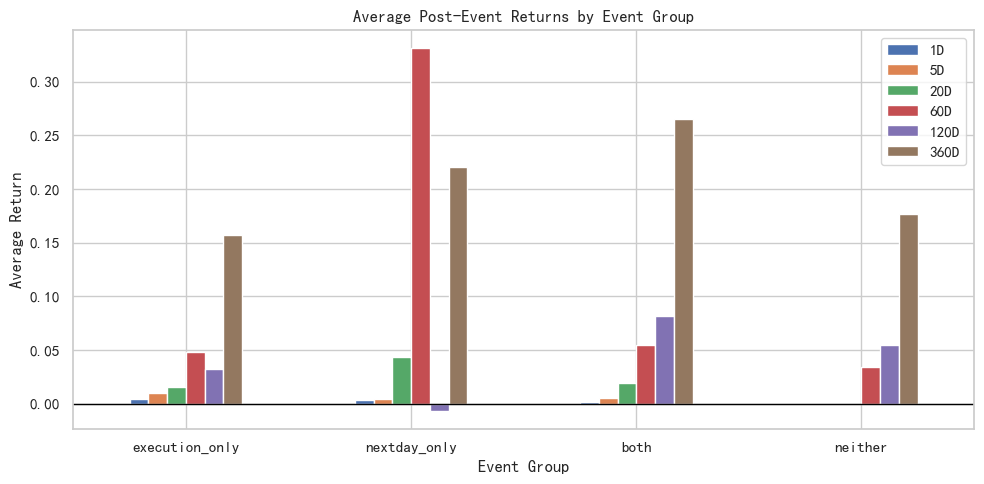
\includegraphics[width=0.9\linewidth]{未来收益柱状图.png}
    \caption{不同公告事件组在多个持有期上的平均未来收益。图中比较了 \texttt{execution\_only}、\texttt{nextday\_only}、\texttt{both} 与 \texttt{neither} 四类事件组在公告后 1 日、5 日、20 日、60 日、120 日与 360 日窗口上的平均未来收益。整体来看，\texttt{both} 组在中长期窗口上的收益表现相对更强，表明同时包含执行信息与翌日披露属性的公告可能具有更高的信息含量。\texttt{nextday\_only} 组由于样本量极小，其结果仅供探索性参考。}
    \label{fig:avg_post_event_returns}
\end{figure}




\begin{table}[H]
\centering
\caption{不同公告事件组相对于 \texttt{neither} 组的未来收益均值差异检验}
\label{tab:mean_diff_test}
\resizebox{\textwidth}{!}{
\begin{tabular}{l l r r r r r}
\toprule
\textbf{事件组别} & \textbf{持有期} & \textbf{组均值} & \textbf{基准组均值} & \textbf{均值差} & \textbf{t统计量} & \textbf{p值} \\
\midrule
\texttt{execution\_only} & 60日  & 0.0479 & 0.0345 & 0.0134  & 1.2047  & 0.2284 \\
\texttt{execution\_only} & 120日 & 0.0323 & 0.0545 & -0.0222 & -2.1553 & 0.0312 \\
\texttt{execution\_only} & 360日 & 0.1570 & 0.1766 & -0.0196 & -0.7829 & 0.4338 \\
\midrule
\texttt{nextday\_only}   & 60日  & 0.3310 & 0.0345 & 0.2965  & 7.1101  & 0.0001 \\
\texttt{nextday\_only}   & 120日 & -0.0069 & 0.0545 & -0.0614 & -3.1404 & 0.0200 \\
\texttt{nextday\_only}   & 360日 & 0.2209 & 0.1766 & 0.0443  & 2.0198  & 0.0896 \\
\midrule
\texttt{both}            & 60日  & 0.0550 & 0.0345 & 0.0205  & 8.5885  & 0.0000 \\
\texttt{both}            & 120日 & 0.0819 & 0.0545 & 0.0274  & 10.1879 & 0.0000 \\
\texttt{both}            & 360日 & 0.2653 & 0.1766 & 0.0887  & 9.8584  & 0.0000 \\
\bottomrule
\end{tabular}
}
\begin{tablenotes}
\small
\item 注：表中将 \texttt{execution\_only}、\texttt{nextday\_only} 与 \texttt{both} 三类事件组分别与 \texttt{neither} 组进行未来收益均值差异检验。\texttt{neither} 组作为基准组，代表未命中核心执行型公告标签组合的样本。由于短期收益窗口中存在异常值问题，本文仅报告 60 日、120 日与 360 日持有期的检验结果。从结果看，\texttt{both} 组在三个中长期窗口上均显著高于基准组，说明同时包含执行信息与翌日披露属性的公告，可能具有更强的信息含量。\texttt{nextday\_only} 组样本量极小，因此其显著性结果需谨慎解读。
\end{tablenotes}
\end{table}


在实证呈现上，本文首先对不同事件组的未来收益进行了描述性统计。结果显示，四类事件组在样本分布与收益表现上存在明显差异。就样本规模而言，\texttt{neither} 组占据绝大多数股票--日期观测，而真正具有核心回购执行属性的事件样本主要集中于 \texttt{both} 组（即同时命中 \texttt{execution} 与 \texttt{nextday} 标签），其样本量显著高于 \texttt{execution\_only} 与 \texttt{nextday\_only}。这一分布特征表明，在实际公告披露中，“翌日披露”往往并非独立出现，而是通常与执行类表述共同出现，因此同时具备两类语义特征的公告构成了最具代表性的核心事件样本。

从未来收益的均值表现来看，不同公告组在中长期窗口上的差异较为明显。具体而言，\texttt{both} 组在 60 日、120 日与 360 日窗口上的平均未来收益分别达到 5.50\%、8.19\% 与 26.53\%，整体高于 \texttt{execution\_only} 组以及基准组 \texttt{neither}。相比之下，\texttt{execution\_only} 组虽然在短中期也呈现正收益，但其持续性与强度均相对较弱；而 \texttt{nextday\_only} 组虽然在部分窗口中表现出较高收益，但由于样本量极小，仅能作为探索性结果加以参考，不能据此做出稳健推断。总体而言，描述统计结果初步表明：\textbf{同时包含“执行信息”与“翌日披露属性”的公告，可能比单一类型公告具有更强的信息含量与更持续的市场影响。}

在此基础上，本文进一步将各事件组与基准组 \texttt{neither} 进行均值差异比较，以更系统地评估不同公告类别的市场反应差异。检验结果显示，\texttt{both} 组在 60 日、120 日与 360 日三个中长期窗口上的未来收益均显著高于基准组，且统计显著性较强；这意味着，当一则公告同时具备“回购执行”与“翌日披露”两类特征时，市场往往会在随后较长时间内给予更为积极的价格反应。相比之下，\texttt{execution\_only} 组相对于基准组的超额收益并不稳定，在部分窗口中甚至弱于基准组；而 \texttt{nextday\_only} 组虽然在个别窗口中呈现显著差异，但考虑到其极小的样本规模，相关结果应谨慎解读。因此，从“信息含量筛查”的角度看，\texttt{both} 组是当前样本中最值得进一步关注的核心公告类型。

除了若干固定持有期上的离散收益外，本文还进一步构建了事件后累计收益路径，以观察不同公告组在更连续时间维度上的价格演化特征。具体而言，以公告日为基点，沿事件后第 \(0\) 至第 \(H\) 个交易日逐步计算累计收益，并在组内取横截面平均，从而得到不同公告类别的平均事件后价格路径。相较于仅比较若干离散持有期收益，这种路径分析能够更直观地揭示：市场对某类公告的反应究竟是在公告后短期内迅速完成，还是在更长时间窗口内持续释放。结合当前均值统计结果，预计 \texttt{both} 组更可能呈现出相对平稳且持续上升的收益路径，而非一次性的短期跳升。

这一部分分析的意义主要体现在两个方面。第一，它将原本停留在公告标题层面的文本标签，转化为可以直接进入收益检验的事件变量，从而将文本识别、事件研究与资产定价分析有效连接起来。第二，当前结果已经显示，不同公告类别之间确实存在系统性的未来收益差异，尤其是同时包含执行与翌日披露特征的公告，可能携带更强的增量信息。这为后续将公告类别与连续型股东回报指标（如股息率、回购强度以及综合 shareholder return 指标）结合，构建更具解释力的增强型股东回报因子，提供了明确的经验基础。








\section{股息回购交叉分组视角下的股东回报信号检验}

在前文完成基础变量构造后，本文进一步从股票层面的长期特征出发，对样本股票进行分组，并在组内分别检验股息率与回购收益率信号的预测能力。该部分分析的核心目的在于回答：\textbf{当股票在“分红覆盖”与“回购活跃度”两个维度上存在结构性差异时，不同股东回报指标的有效性是否会发生系统性变化。}

与直接在全样本上检验单一因子不同，这一部分更关注股东回报信号的\textbf{适用边界（boundary condition）}。若某一类信号仅在特定股票组中表现有效，则说明其经济含义可能并非普适性的横截面定价因子，而更接近于一种依赖股票特征的条件性信息变量。这样的分组分析不仅有助于理解不同股东回报方式背后的经济机制，也能够为后续综合因子的构造提供更有针对性的依据。

\subsection{股票分组方法}

本文首先在股票层面构造两个用于分组的长期统计量。第一类统计量是股票在样本期内的\textbf{回购活跃度}，以回购公告或回购发生次数（\texttt{buyback\_count}）衡量；第二类统计量是股票\textbf{股息率信息的可得程度}，以股息率非缺失观测的出现次数（\texttt{dy\_count}）衡量。前者反映公司是否长期倾向于通过回购向股东返还现金，后者则刻画股票是否具有相对稳定、可持续追踪的股息率信息。

在此基础上，本文分别按照两个统计量的横截面分位数设定阈值，并据此将样本股票划分为四个组别：
\begin{itemize}
    \item \texttt{both\_top}：回购活跃度与股息率覆盖度均较高；
    \item \texttt{buyback\_only}：仅回购活跃度较高；
    \item \texttt{dy\_only}：仅股息率覆盖度较高；
    \item \texttt{neither}：两者均不突出。
\end{itemize}

这一分组方式本质上是在股票层面构造一个“股东回报风格”的二维划分框架。直观上，\texttt{both\_top} 组更可能包含同时具有稳定分红政策与持续回购行为的成熟公司；\texttt{buyback\_only} 组则更接近以回购为主要股东回报工具的股票；\texttt{dy\_only} 组则更可能对应传统高分红股票；而 \texttt{neither} 组则反映在两类股东回报维度上都不突出的公司。通过在这些组别中分别检验信号有效性，可以更清晰地观察不同股东回报变量在不同股票生态中的作用方式。





\subsection{分位数阈值的敏感性检验}

由于四象限分组依赖于对 \texttt{buyback\_count} 与 \texttt{dy\_count} 所设定的横截面分位数阈值，因此有必要进一步考察：前文关于不同组别中股东回报信号有效性的结论，是否会随着阈值变化而发生明显改变。若结论仅在某一组特定阈值下成立，则说明其更可能是分组方式带来的样本偶然性；反之，若在一系列相近阈值设定下都能重复观察到相似模式，则说明其具有更强的稳健性。

为此，本文进一步对分组阈值进行了系统性的敏感性检验。具体而言，分别对 \texttt{buyback\_count} 与 \texttt{dy\_count} 设定多个候选分位点，并在不同阈值组合下重复构造 \texttt{both\_top}、\texttt{buyback\_only}、\texttt{dy\_only} 与 \texttt{neither} 四类股票组别，再在组内重新计算股息率与回购收益率信号的 Rank IC 表现。与此同时，考虑到极端低流动性股票可能放大噪音，本文在该部分检验中进一步加入了年度流动性筛选：对每一年，仅保留当年日均成交额（\texttt{amount}）位于样本前 $50\%$ 的股票，以提高组内比较的可解释性。

\begin{table}[H]
\centering
\caption{不同分位数设定下回购收益率信号的最优表现}
\label{tab:quantile_sensitivity_by}
\small
\begin{tabular}{cccccc}
\toprule
因子 & buyback\_q & dy\_q & 组别 & IC mean & $t$-stat \\
\midrule
BY$_{120}$ & 0.80 & 0.80 & both\_top & 0.0214 & 3.27 \\
BY$_{120}$ & 0.75 & 0.80 & both\_top & 0.0200 & 3.35 \\
BY$_{120}$ & 0.70 & 0.80 & both\_top & 0.0170 & 3.06 \\
BY$_{360}$ & 0.75 & 0.80 & both\_top & 0.0173 & 2.93 \\
BY$_{360}$ & 0.80 & 0.80 & both\_top & 0.0164 & 2.58 \\
BY$_{360}$ & 0.70 & 0.80 & both\_top & 0.0150 & 2.71 \\
\bottomrule
\end{tabular}
\end{table}


从结果来看，回购收益率信号在 \texttt{both\_top} 组中的优势具有较强稳健性。以短期回购收益率 \texttt{by\_120} 为例，其表现最好的若干阈值组合全部集中在 \texttt{both\_top} 组。其中，当 \texttt{buyback\_q}=0.80、\texttt{dy\_q}=0.80 时，\texttt{by\_120} 的平均 IC 达到 $0.0214$，$t$ 统计量为 $3.27$；当 \texttt{buyback\_q}=0.75、\texttt{dy\_q}=0.80 时，平均 IC 为 $0.0200$，$t$ 统计量进一步提高至 $3.35$；即便将回购阈值放宽至 $0.70$，在 \texttt{dy\_q}=0.80 的设定下，\texttt{by\_120} 仍有 $0.0170$ 的平均 IC 与超过 $3$ 的 $t$ 值。类似地，对于中期回购收益率 \texttt{by\_360}，表现最优的设定同样集中于 \texttt{both\_top} 组，且最优组合出现在 \texttt{buyback\_q}=0.75、\texttt{dy\_q}=0.80，其平均 IC 为 $0.0173$，$t$ 统计量为 $2.93$；在 \texttt{buyback\_q}=0.80、\texttt{dy\_q}=0.80 下，\texttt{by\_360} 的平均 IC 也仍达到 $0.0164$，对应 $t$ 值约为 $2.58$。

这些结果说明，\textbf{双高组中回购收益率信号更有效}这一结论并不是由某一个特定阈值“碰巧”驱动出来的，而是在一系列相近且合理的分位数设定下都能够重复观察到。尤其值得注意的是，较优结果大多集中在 \texttt{dy\_q}=0.80 的设定附近，这表明当“高股息率覆盖度”的定义更严格时，\texttt{both\_top} 组的风格识别更清晰，组内回购信号的预测能力也更容易显现出来。相比之下，\texttt{buyback\_q} 从 $0.70$ 到 $0.80$ 的变化虽然会影响样本数，但并未改变回购信号在 \texttt{both\_top} 组中占优的基本事实。

进一步考察代表性阈值组合也可以看到这种稳定模式。当采用较严格的基准设定 \texttt{buyback\_q}=0.80、\texttt{dy\_q}=0.80 时，\texttt{both\_top} 组中 \texttt{by\_120} 与 \texttt{by\_360} 分别取得 $0.0214$ 与 $0.0164$ 的平均 IC，明显优于同组内的各类 DY 信号，而 \texttt{dy\_ffill} 及其平滑版本的 IC 均接近于零甚至略为负值。与此同时，\texttt{dy\_only} 组中则呈现相反格局：\texttt{dy\_20}、\texttt{dy\_60} 与 \texttt{dy\_ffill} 的平均 IC 分别达到 $0.0182$、$0.0175$ 与 $0.0181$，对应的 $t$ 统计量均在 $4.5$ 以上，而回购收益率变量整体较弱。也就是说，在最严格的双 $0.8$ 阈值下，仍然能够清晰观察到“\texttt{both\_top} 组中 BY 占优、\texttt{dy\_only} 组中 DY 占优”的镜像结构。

当阈值略微放宽为 \texttt{buyback\_q}=0.75、\texttt{dy\_q}=0.80 后，这一模式不仅没有消失，反而在一定程度上变得更加平衡：\texttt{both\_top} 组的股票数由 $40$ 只增加至 $47$ 只，\texttt{by\_120} 与 \texttt{by\_360} 依然分别实现 $0.0200$ 与 $0.0173$ 的平均 IC；\texttt{dy\_only} 组中，\texttt{dy\_ffill} 及其平滑版本仍保持约 $0.018$ 左右的平均 IC 和显著的 $t$ 统计量；\texttt{neither} 组中 DY 信号则呈现小幅但相对稳定的正向预测能力。这表明，相较于完全严格的双 $0.8$ 设定，\texttt{buyback\_q}=0.75、\texttt{dy\_q}=0.80 在保留风格差异的同时，还能够提供略高一些的样本覆盖，因此可以视为一个在“分组纯度”与“统计稳定性”之间较为平衡的候选设定。

不过，敏感性检验也显示，不是所有组别的结论都同样稳定。相较于 \texttt{both\_top} 与 \texttt{dy\_only} 两组中清晰且可重复的信号差异，\texttt{buyback\_only} 组中的结果明显更依赖于具体阈值设定。在若干代表性组合下，该组的回购收益率虽仍为正，但显著性明显弱于 \texttt{both\_top} 组；而 \texttt{neither} 组则更多表现为弱信号环境，其结果对分组边界和样本构成都更为敏感。这意味着，前文关于“回购型股票中回购信号更强”的结论，在经验上主要是由 \texttt{both\_top} 这一类同时具备较强股东回报特征的股票所支撑，而非均匀地存在于所有含回购特征的组别中。

总体而言，分位数阈值的敏感性检验进一步支持了本文的核心发现：\textbf{股东回报信号的有效性具有显著的风格依赖性，而这种依赖性在不同合理阈值设定下总体上是稳定存在的。} 更具体地说，\texttt{both\_top} 组中回购收益率持续占优，\texttt{dy\_only} 组中股息率持续占优，这一结构性结果并不依赖于某一个单点阈值设定。相比之下，\texttt{buyback\_only} 与 \texttt{neither} 组的结论则更容易受到样本规模与分组边界的影响。由此可见，四象限分组的价值不在于寻找某一个“最优分位点”，而在于揭示：不同股票所处的分红—回购风格位置，会系统性地改变股东回报信号的有效性。











\subsection{组内信号构造}

在组内因子构造上，本文分别将股息率（Dividend Yield, DY）与回购收益率（Buyback Yield, BY）视为两类经济属性不同的信号。

首先，股息率被视为一种相对缓慢变化的\textbf{状态变量}。由于港股股息率披露频率较低，但其经济含义通常具有一定持续性，本文对个股股息率序列进行前向填充（forward fill），构造连续的日频股息率变量 \texttt{dy\_ffill}，并在每日横截面内进行排序，形成股息率排序信号。这样的处理方式旨在尽可能保留股息政策的持续信息，同时避免因原始披露稀疏而导致的大量无效观测。

其次，股票回购被视为一种更具事件性和流量属性的\textbf{流量变量}。本文先将每日回购金额缺失值视为零，再分别在 $120$、$360$ 和 $720$ 个交易日窗口内构造滚动累计回购金额，并除以当期市值，得到不同期限下的回购收益率变量 \texttt{by\_120}、\texttt{by\_360} 和 \texttt{by\_720}。这一处理方式意在将离散发生的回购行为转化为具有可比性的持续型指标，从而便于与股息率信号进行统一比较。

在此基础上，本文还进一步构造综合性的\textbf{股东回报收益率（shareholder yield）}：
\[
\text{Shareholder Yield} = \text{Dividend Yield} + \text{Buyback Yield},
\]
分别得到 \texttt{shy\_120}、\texttt{shy\_360} 与 \texttt{shy\_720}。这一指标的含义在于，将企业通过现金分红与股票回购两种方式向股东返还价值的行为统一纳入同一框架，从而检验“总股东回报”这一更综合的资本分配信号是否比单一分红或单一回购更具解释力。

\subsection{检验方法与有效样本问题}

本文在组内采用逐日横截面排序检验的方法评估信号有效性。具体而言，对于每一交易日，先在组内对候选因子进行横截面排序，再计算其与下一期收益（\texttt{ret\_next}）之间的 Spearman Rank IC，最后在时间维度上汇总其均值、标准差以及 $t$ 统计量，用以衡量该信号在组内的平均预测能力及统计显著性。

需要特别指出的是，不同组别之间的\textbf{有效横截面股票数}存在明显差异，而这会直接影响组内 IC 的稳定性与可解释性。为了避免将统计噪音误判为经济信号，本文进一步统计了每个组别、每个因子在每日横截面中的有效股票数分布。

结果显示，不同组别在有效样本覆盖上存在显著异质性。对于 \texttt{both\_top} 组，\texttt{dy\_cs\_ffill} 的日均有效股票数约为 $80.5$ 只，而三个回购收益率变量的日均有效股票数均约为 $85.9$ 只，说明该组在两类股东回报维度上都具有较好的信息覆盖度，因此是最适合进行“股东回报综合比较”的样本组。相对而言，\texttt{dy\_only} 组在样本覆盖上甚至更强，\texttt{dy\_cs\_ffill} 的日均有效股票数达到约 $135.2$ 只，回购收益率变量也有约 $127.2$ 只，说明即便这些股票在长期上不属于“回购活跃型”，其横截面中仍然保留了足够多的回购信息用于比较。

但在 \texttt{buyback\_only} 组与 \texttt{neither} 组中，股息率信号的有效样本问题则非常突出。具体来看，\texttt{buyback\_only} 组中 \texttt{dy\_cs\_ffill} 的日均有效股票数仅约为 $1.58$ 只，而 \texttt{neither} 组也仅约为 $4.81$ 只。这意味着在这两个组别中，股息率横截面排序几乎无法形成具有经济含义的截面比较，因此其 IC 结果应谨慎解读。相比之下，回购收益率变量在这两个组别中的横截面规模仍分别达到约 $17.0$ 只与 $44.0$ 只，尽管不算很大，但仍明显优于股息率变量。因此，从方法上看，后续对于 \texttt{buyback\_only} 与 \texttt{neither} 组的结论应更多依赖回购相关信号，而不宜过度依赖股息率指标。

\subsection{分组结果：股息率与回购收益率的相对表现}

在单一信号的组内表现上，结果呈现出较为清晰的结构性差异。


\begin{table}[H]
\centering
\caption{各组别下不同股东回报信号的组内 IC 表现}
\label{tab:group_ic_results}
\small
\begin{tabular}{llccccccc}
\toprule
组别 & 统计量 & DY & BY$_{120}$ & BY$_{360}$ & BY$_{720}$ & SHY$_{120}$ & SHY$_{360}$ & SHY$_{720}$ \\
\midrule

\multirow{2}{*}{both\_top}
& IC mean & 0.0037 & 0.0116 & 0.0079 & 0.0004 & 0.0041 & 0.0041 & 0.0041 \\
& $t$-stat & 0.98 & 2.62 & 1.85 & 0.09 & 1.10 & 1.10 & 1.09 \\

\midrule

\multirow{2}{*}{buyback\_only}
& IC mean & -0.0509 & 0.0289 & 0.0215 & 0.0277 & -0.0094 & -0.0108 & -0.0097 \\
& $t$-stat & -1.74 & 2.98 & 2.10 & 2.67 & -0.90 & -1.04 & -0.94 \\

\midrule

\multirow{2}{*}{dy\_only}
& IC mean & 0.0146 & -0.0097 & -0.0070 & -0.0032 & 0.0129 & 0.0130 & 0.0130 \\
& $t$-stat & 4.34 & -2.47 & -1.74 & -0.85 & 3.92 & 3.92 & 3.92 \\

\midrule

\multirow{2}{*}{neither}
& IC mean & 0.0164 & 0.0069 & 0.0068 & 0.0140 & 0.0114 & 0.0114 & 0.0127 \\
& $t$-stat & 1.11 & 1.04 & 1.13 & 2.37 & 2.40 & 2.42 & 2.69 \\

\bottomrule
\end{tabular}
\vspace{0.5em}
\begin{minipage}{0.92\textwidth}
\footnotesize
\textit{Notes:} DY 表示前向填充后的股息率信号；BY$_{120}$、BY$_{360}$、BY$_{720}$ 分别表示以 120、360 和 720 个交易日滚动累计回购金额除以当期市值得到的回购收益率；SHY 为 shareholder yield，即 DY 与对应 BY 的加总。表中报告各组别内逐日横截面 Spearman Rank IC 的时间序列均值与对应 $t$ 统计量。
\end{minipage}
\end{table}




首先，在 \texttt{both\_top} 组中，回购收益率信号整体优于股息率信号。具体而言，\texttt{dy\_ffill} 的平均 IC 仅为 $0.0037$，且 $t$ 统计量不足 $1$，预测能力较弱；相比之下，\texttt{by\_120} 的平均 IC 达到 $0.0116$，对应 $t$ 统计量约为 $2.62$，表现最为突出，\texttt{by\_360} 亦维持正向且边际显著。

这说明在同时具备高分红与高回购特征的股票中，市场对“近期回购强度”的反应可能比对静态股息率水平更敏感。换言之，对于这类本身已具有较高股东回报属性的公司而言，\textbf{新增的回购流量信息}可能比\textbf{已被市场较充分认知的分红状态信息}更能提供增量预测内容。

其次，在 \texttt{buyback\_only} 组中，这一特征表现得更为明显。该组中 \texttt{by\_120}、\texttt{by\_360} 与 \texttt{by\_720} 的平均 IC 分别约为 $0.0289$、$0.0215$ 与 $0.0277$，对应的 $t$ 统计量均在 $2$ 左右或以上，显示出较为稳定的正向预测能力。相反，\texttt{dy\_ffill} 的 IC 为负，且由于横截面有效股票数极低，其结果本身并不具备可靠的经济解释。这一结果与该组的定义高度一致：对于本身更依赖回购而非分红进行股东回报的股票而言，\textbf{回购收益率确实是更自然、更有效的信号载体}。

再次，在 \texttt{dy\_only} 组中，结果则呈现出明显的镜像结构。该组中 \texttt{dy\_ffill} 的平均 IC 为 $0.0146$，对应 $t$ 统计量约为 $4.34$，显著优于同组内所有回购收益率变量；而 \texttt{by\_120}$ 和 \texttt{by\_360}$ 的平均 IC 甚至为负。这意味着在传统高分红型股票中，股息率本身依然保留了较强的横截面预测能力，而回购行为不仅信息含量有限，甚至可能带来噪音。这一结果说明，\textbf{股东回报信号具有明显的“同源性”特征：分红型股票中，分红信号有效；回购型股票中，回购信号有效。}

最后，在 \texttt{neither} 组中，单一信号整体表现较弱，但长期回购收益率仍显示出一定解释力。具体而言，\texttt{dy\_ffill} 的平均 IC 为 $0.0164$，但其横截面有效样本数较低，解释空间有限；而 \texttt{by\_720} 的平均 IC 达到 $0.0140$，对应 $t$ 统计量约为 $2.37$，在三个回购窗口中表现最好。这表明对于那些既不属于高分红、也不属于高回购的“边缘型”股票而言，短期股东回报行为可能较为噪音化，但\textbf{较长期累计的回购行为}仍可能携带一定的估值修复或资本配置含义。

综合来看，单一信号的组内检验结果呈现出较强的结构一致性：\texttt{buyback\_only} 与 \texttt{both\_top} 组中，回购收益率相对更有效；\texttt{dy\_only} 组中，股息率显著占优；\texttt{neither} 组则更偏向于长期回购信号。这一结果说明，股东回报信号并不存在单一“统治性”变量，其有效性很大程度上取决于股票本身的股东回报风格。

\subsection{分组结果：Shareholder Yield 是否优于单一信号}

在将股息率与回购收益率加总构造为 shareholder yield 后，结果显示这一综合指标并不总是优于单一信号，其表现同样具有明显的组别依赖性。

\begin{table}[H]
\centering
\caption{各组别下 DY、最佳 BY 与最佳 SHY 的表现对比}
\label{tab:dy_by_shy_compare}
\small
\begin{tabular}{lcccccc}
\toprule
组别 & DY IC & DY $t$ & 最佳 BY IC & 最佳 BY $t$ & 最佳 SHY IC & 最佳 SHY $t$ \\
\midrule
\texttt{both\_top}     & 0.0251  & 9.22 & 0.0116  & 2.62 & 0.0247  & 9.49 \\
\texttt{buyback\_only} & -0.0509 & -1.74 & 0.0289  & 2.98 & -0.0094 & -0.90 \\
\texttt{dy\_only}      & 0.0146  & 4.34 & -0.0032 & -0.85 & 0.0130  & 3.92 \\
\texttt{neither}       & 0.0164  & 1.11 & 0.0140  & 2.37 & 0.0127  & 2.69 \\
\bottomrule
\end{tabular}
\vspace{0.5em}
\begin{minipage}{0.9\textwidth}
\footnotesize
\textit{Notes:} “最佳 BY”表示 \texttt{by\_120}、\texttt{by\_360} 与 \texttt{by\_720} 中 IC mean 最高者；“最佳 SHY”表示 \texttt{shy\_120}、\texttt{shy\_360} 与 \texttt{shy\_720} 中 IC mean 最高者。该表用于比较综合性 shareholder yield 指标与单一分红、单一回购信号在不同股票组别中的相对有效性。
\end{minipage}
\end{table}

对于 \texttt{both\_top} 组，\texttt{shy\_120}、\texttt{shy\_360} 与 \texttt{shy\_720} 的平均 IC 均约为 $0.0041$ 左右，整体明显弱于 \texttt{by\_120} 本身。这说明在高分红且高回购股票中，简单地将两类信号线性叠加，并未显著提升预测能力，反而可能在一定程度上稀释了原本更强的回购信息。换言之，在这一组中，\textbf{“总股东回报”并不优于“边际回购变化”}。

在 \texttt{buyback\_only} 组中，这种“稀释效应”更加明显。虽然单独的回购收益率信号具有较好的正向 IC，但 \texttt{shy\_120}、\texttt{shy\_360} 与 \texttt{shy\_720} 的平均 IC 均转为小幅负值，且统计上不显著。这意味着在本就缺乏稳定分红信息的股票中，将一个噪音较大的股息率变量与有效的回购收益率简单相加，反而会削弱因子整体表现。也就是说，\textbf{在“单一回购型”股票中，shareholder yield 的概念上虽更完整，但在实证上未必更优。}

然而，在 \texttt{dy\_only} 组中，shareholder yield 则表现出一定的稳健性。该组中 \texttt{shy\_120}、\texttt{shy\_360} 与 \texttt{shy\_720} 的平均 IC 均约为 $0.013$ 左右，对应的 $t$ 统计量接近或超过 $4$，整体与 \texttt{dy\_ffill} 非常接近。这说明在高分红股票中，加入回购收益率后并未明显破坏原有的分红信号，综合指标仍保留了较好的预测能力。不过需要指出的是，这种表现更可能来自\textbf{DY 本身的主导作用}，而非回购信息提供了显著增量。

在 \texttt{neither} 组中，shareholder yield 反而显示出相对更好的综合表现。该组中 \texttt{shy\_120}、\texttt{shy\_360} 与 \texttt{shy\_720} 的平均 IC 分别约为 $0.0114$、$0.0114$ 与 $0.0127$，对应的 $t$ 统计量均在 $2.4$ 至 $2.7$ 左右，整体优于组内大多数单一变量。这一结果表明，在两类股东回报特征都不突出的股票中，单独使用某一维度的信号可能信息不足，而\textbf{将两类弱信号进行合成}反而能够提炼出一定的共同有效信息。这可能意味着，shareholder yield 在“非典型股东回报型”股票中，具有更高的适配性。

总体而言，shareholder yield 的组内表现说明：\textbf{“综合”并不天然优于“专门化”}。当某一股票组本身具有明确的股东回报主导方式时，使用对应的单一信号往往更有效；而当股票缺乏明确的分红或回购特征时，综合性指标反而更有可能发挥作用。因此，shareholder yield 更适合作为一种\textbf{条件性补充信号}，而非简单地在所有股票上替代分红率或回购收益率。

\subsection{小结}

本节从股票长期特征出发，对样本进行了基于“回购活跃度”和“股息率覆盖度”的二维分组，并在组内比较了股息率、回购收益率以及 shareholder yield 的预测能力。结果表明，不同股东回报信号的有效性具有显著的组别依赖性，且这种异质性与股票本身的股东回报风格高度一致。

更具体地说，在回购特征更强的股票中，回购收益率信号更具解释力；在分红特征更强的股票中，股息率信号更有效；而在两类特征都不突出的股票中，综合性的 shareholder yield 反而表现出更好的稳健性。这一发现说明，股东回报因子的构造不宜简单依赖统一口径，而更应考虑股票在分红与回购维度上的结构性差异。

因此，从后续因子设计的角度看，一个自然的延伸方向并不是在全样本上机械地使用统一的 shareholder yield 指标，而是考虑引入\textbf{分组加权、条件切换或风格适配}的构造方式，使股东回报信号在不同类型股票中以更贴合其经济属性的形式发挥作用。










\section{基于公告语义重分类的股东回报信号检验}

除了基于股票长期特征进行分组外，本文进一步尝试从\textbf{公告语义与执行属性}出发，对回购相关事件进行重新分类，并考察在不同公告类别下，股息率与回购收益率信号的预测能力是否存在系统性差异。与前文基于股票“长期风格特征”的分组不同，本部分更强调\textbf{事件本身的信息结构}，即不同类型的回购公告是否携带不同程度、不同方向的资本分配信息。

这一扩展分析的动机在于：股票回购并非单一、同质的行为。即便都属于“回购相关公告”，其背后所反映的经济含义也可能显著不同。例如，有些公告更接近于\textbf{实际执行层面的现金返还行为}，而另一些则可能仅仅反映董事会授权、程序推进或未来计划，并不一定对应立即发生的资本流出。因此，若将所有回购公告简单合并，可能会掩盖不同事件类别之间真实的信息异质性。

\subsection{公告语义重分类方法}

本文在原始公告文本分类的基础上，进一步聚焦于与股票回购最相关的几类事件，并据此重新构造四类事件组：
\begin{itemize}
    \item \texttt{execution\_only}：仅包含“实际执行回购”特征的公告；
    \item \texttt{nextday\_only}：仅包含“次日执行安排或执行预告”特征的公告；
    \item \texttt{both}：同时具备“执行”与“次日执行安排”特征的公告；
    \item \texttt{neither}：不属于上述两类核心执行型特征的其他公告。
\end{itemize}

这一分类方式试图区分\textbf{真正发生的回购行为}与\textbf{尚停留在预告、安排或程序性层面}的公告。直观而言，\texttt{execution\_only} 更可能对应公司已经发生的现金回购行为，因此其信息含量应更接近真实资本分配动作；\texttt{nextday\_only} 则更偏向于计划性或预告性信息，其是否能够转化为市场定价信号，本身并不确定；\texttt{both} 则可能反映“已执行且持续推进”的回购进程；而 \texttt{neither} 则更多包含授权、完成、一般性说明或其他弱执行属性的回购公告。

与前文股票层面的风格分组不同，这一分类更强调\textbf{事件驱动的异质性}，因此其本质上是在检验：\textbf{回购公告的“内容类型”是否决定了股东回报信号的有效性。}

\subsection{因子构造与检验设计}

在信号构造上，本文延续前文的处理方式，分别考察股息率与回购收益率两类股东回报指标。

首先，股息率信号继续采用前向填充后的 \texttt{dy\_ffill}，并在每日横截面中进行排序，以反映股票在分红维度上的相对状态。其次，回购收益率信号仍定义为不同滚动窗口下累计回购金额除以当期市值，分别构造 \texttt{by\_120}、\texttt{by\_360} 和 \texttt{by\_720} 三个版本，用以捕捉短、中、长期累计回购强度。

在检验方法上，本文同样采用组内逐日横截面 Spearman Rank IC 的方式，对因子值与下一期收益之间的秩相关关系进行评估，并报告时间序列上的 IC 均值、标准差、$t$ 统计量及有效观测天数 $N$。这一检验框架能够较为直接地识别：在不同类型的回购公告环境中，究竟是股息率信号、回购收益率信号，还是两者均不具备稳定的预测能力。

\begin{table}[H]
\centering
\caption{基于公告语义重分类的组内 IC 结果}
\label{tab:semantic_group_ic}
\small
\begin{tabular}{llcccc}
\toprule
组别 & 统计量 & DY & BY$_{120}$ & BY$_{360}$ & BY$_{720}$ \\
\midrule

\multirow{2}{*}{execution\_only}
& IC mean & 0.0256 & -0.0187 & -0.0187 & -0.0187 \\
& $t$-stat & 2.89 & -0.32 & -0.32 & -0.32 \\

\midrule

\multirow{2}{*}{nextday\_only}
& IC mean & -- & -- & -- & -- \\
& $t$-stat & -- & -- & -- & -- \\

\midrule

\multirow{2}{*}{both}
& IC mean & 0.0297 & 0.0067 & 0.0177 & 0.0185 \\
& $t$-stat & 1.88 & 0.46 & 1.25 & 1.33 \\

\midrule

\multirow{2}{*}{neither}
& IC mean & 0.0115 & -0.0023 & 0.0001 & 0.0013 \\
& $t$-stat & 3.52 & -0.86 & 0.03 & 0.49 \\

\bottomrule
\end{tabular}
\vspace{0.5em}
\begin{minipage}{0.9\textwidth}
\footnotesize
\textit{Notes:} 本表报告基于公告语义重分类后的组内因子表现。DY 表示前向填充后的股息率信号，BY 表示不同滚动窗口下的回购收益率信号。组别依据公告文本是否包含“实际执行”与“次日执行安排”特征构造。表中报告逐日横截面 Spearman Rank IC 的时间序列均值与对应 $t$ 统计量。
\end{minipage}
\end{table}

\subsection{结果一：执行型公告组中的股息率信号更强}

实证结果显示，在 \texttt{execution\_only} 组中，股息率信号表现出极强的正向预测能力，而回购收益率信号则并未体现出相应优势。具体而言，\texttt{dy\_ffill} 的平均 IC 达到 $0.2567$，对应 $t$ 统计量约为 $2.89$，显著高于其他因子；相比之下，\texttt{by\_120}、\texttt{by\_360} 与 \texttt{by\_720} 的平均 IC 均为约 $-0.0187$ ，不仅方向为负，且统计上完全不显著。

这一结果具有一定的经济含义。表面上看，\texttt{execution\_only} 组似乎应最适合回购收益率信号发挥作用，因为其公告本身更接近真实回购执行行为。然而实证结果恰恰表明，\textbf{真正发生执行型回购的股票，可能本身就是一类具有较强股东回报属性的公司，而这种属性更早、更稳定地体现在股息率水平中，而不是体现在短期滚动回购金额中。}换言之，市场对“执行型回购”的定价，可能并不是通过短期回购流量本身完成的，而是通过对公司整体资本分配风格的再识别来完成的。

当然，也需要指出，该组的样本规模相对较小（\texttt{dy\_ffill} 对应 $N=89$，回购收益率对应 $N=143$），因此这一结果虽然方向上较为鲜明，但仍应视为一种具有启发性的证据，而非最终定论。

\subsection{结果二：混合执行组中，回购信号略有改善但整体有限}

在 \texttt{both} 组中，即同时具备“执行”与“次日执行安排”特征的公告组，结果显示股息率与回购收益率信号均表现为弱正向，但整体强度有限。

其中，\texttt{dy\_ffill} 的平均 IC 为 $0.0297$，对应 $t$ 统计量约为 $1.88$，在统计上接近边际显著；而 \texttt{by\_120}$、\texttt{by\_360}$ 与 \texttt{by\_720} 的平均 IC 分别为 $0.0067$、$0.0177$ 与 $0.0185$，均为正值，但对应的 $t$ 统计量仍不足以支持其具有稳定显著性。

与 \texttt{execution\_only} 组相比，这一结果说明：当回购公告同时包含执行与后续安排信息时，回购收益率信号确实有所改善，尤其是中长期滚动窗口下的 \texttt{by\_360} 与 \texttt{by\_720}，其 IC 表现已明显好于短期窗口 \texttt{by\_120}。这意味着市场可能更重视“持续性回购进程”所反映的长期资本分配态度，而非单一时点的短期回购金额。然而总体而言，该组结果依然说明，\textbf{即便是在更“强执行属性”的公告环境下，回购收益率信号也并未展现出压倒性的预测优势。}

\subsection{结果三：非执行型公告组中，DY 信号依然更稳健}

在 \texttt{neither} 组中，即不属于“执行”或“次日执行安排”两类核心执行属性的公告组中，股息率信号依然表现出更稳定的预测能力，而回购收益率信号整体接近于零。

具体来看，\texttt{dy\_ffill} 的平均 IC 为 $0.0115$，对应 $t$ 统计量约为 $3.52$，显示出较为稳健的正向预测关系；而 \texttt{by\_120}、\texttt{by\_360} 与 \texttt{by\_720} 的平均 IC 分别约为 $-0.0023$、$0.0001$ 与 $0.0013$，均极为接近零，且统计上不显著。

这一结果表明，即便在那些\textbf{并不直接对应实际执行动作}的回购公告中，股息率所代表的长期资本返还风格仍然具有可识别的横截面信息含量；而公告文本中弱执行属性所对应的回购信息，则很难通过滚动回购收益率变量转化为稳定的收益预测能力。从经济上看，这说明很多“回购相关公告”本身可能更多只是\textbf{制度性、程序性或沟通性披露}，其对市场定价的边际贡献相对有限。

\subsection{结果四：次日执行型公告样本极少，暂不具备可解释性}

在 \texttt{nextday\_only} 组中，本文未获得有效的横截面样本，所有因子的 IC、标准差与 $t$ 统计量均为缺失值，对应有效观测天数 $N=0$。这说明在当前样本和分类规则下，该类公告本身出现频率极低，或其在与日度面板数据匹配后无法形成足够的横截面观测，因此暂不具备独立的统计分析意义。

这一结果本身也具有一定启发性：从市场结构角度看，“仅包含次日执行安排而不包含其他执行信息”的公告可能并不是一个稳定、可重复出现的事件类型，因此在后续研究中，更适合将其并入 broader execution-related 组别，而非单独作为一个可交易信号类别来处理。

\subsection{小结与启示}

总体来看，基于公告语义重分类后的实证结果表明，\textbf{回购公告的“执行属性”确实能够区分不同类型的股票与事件环境，但这种区分并未自动转化为更强的回购收益率信号。}相反，在多数组别中，股息率信号依然表现出更强或更稳健的解释力，而滚动回购收益率变量仅在少数组别中呈现出有限的正向信息。

这一结果对后续因子构造具有两点重要启示。第一，\textbf{回购相关公告的异质性是真实存在的}，因此将所有回购事件视为同质信号可能会削弱因子的经济解释力；第二，\textbf{回购行为本身未必最适合通过简单滚动金额除以市值的方式来度量}。从当前结果看，公告的“是否执行”更多像是一种\textbf{事件筛选维度}，能够帮助识别哪些股票更具有股东回报属性，但其本身并不一定足以让回购收益率成为强预测因子。

因此，一个更自然的后续方向是：在公告语义重分类的基础上，不是直接比较“DY vs. BY”，而是进一步考虑\textbf{事件筛选 + 条件性因子构造}的框架，例如仅在特定执行型公告组中保留回购相关信号，或对不同公告类别采用不同的股东回报指标权重。这将有助于在保留经济解释力的同时，提高因子的实证表现。



























\end{document}
